\documentclass{article}
\usepackage{graphicx}
\usepackage{authblk}
\usepackage{natbib}
\usepackage{hyperref}
\hypersetup{
    colorlinks,
    citecolor=black,
    filecolor=black,
    linkcolor=black,
    urlcolor=black
}

\begin{document}

\title{Supplemental Material for \\ Helixer: Cross-species Gene Annotation of Large Eucaryotic Genomes Using Deep Learning}

\author[1]{Felix Stiehler}
\author[1]{Alisandra Denton}
\author[1]{Marvin Steinborn}
\author[ \hspace{-1ex}]{Stephan Scholz}
\author[1]{Andreas Weber}
\affil[1]{Institue for Plant Biochemistry, Heinrich-Heine-University, Dusseldorf, D-40225, Germany}

%\author[Sample \textit{et~al}.]{Felix Stiehler\,$^{\text{\sfb 1,}}$$^\dagger$, Alisandra Denton\,$^{\text{\sfb 1,}}$$^\dagger$\, Marvin Steinborn\,$^{\text{\sfb 1}}$, Stephan Scholz, Andreas Weber\,$^{\text{\sfb 1,}*}$}
% \address{$^{\text{\sf 1}}$Institue for Plant Biochemistry, Heinrich-Heine-University, Dusseldorf, D-40225, Germany}
% \author{Author's Name}

\date{}
\maketitle
\tableofcontents

\newpage
\section{In-depth model performance}

\begin{table}[!h]
\renewcommand\thetable{S1}
\centering
\begin{tabular}{@{}lll@{}}
\hline
Class & Animal Value & Plant Value \\ [0.5ex]
\hline
Intergenic & 0.7 & 0.3 \\
UTR & 1.6 & 1.0 \\
CDS & 1.2 & 0.9 \\
Intron & 1.2 & 0.3 \\
\hline
\end{tabular}
\caption{}
\end{table}

\newpage
\section{Hyperparameters}

\begin{table}[!h]
\renewcommand\thetable{S1}
\centering
\begin{tabular}{@{}ll@{}}
\hline
Parameter & Value \\ [0.5ex]
\hline
Layers & 4\\
Units per layer & 256\\
Learning rate & 1e-4\\
Optimizer & Adam\\
\hline
\end{tabular}
\caption{All hyperparameters used for the }
\label{suptab:params}
\end{table}

\begin{table}[!h]
\renewcommand\thetable{S1}
\centering
\begin{tabular}{@{}lll@{}}
\hline
Class & Animal Value & Plant Value \\ [0.5ex]
\hline
Intergenic & 0.7 & 0.3 \\
UTR & 1.6 & 1.0 \\
CDS & 1.2 & 0.9 \\
Intron & 1.2 & 0.3 \\
\hline
\end{tabular}
\caption{The class weights are the only hyperparameters that are different for animals and plants. The exact weights were determined manually and partially reflect the difference in the class distributions of both datasets (see Table [?]).}
\end{table}


\newpage
\section{Longer Sequence Input}
\label{sec:longer}
\begin{table}[!h]
\renewcommand\thetable{S1}
\centering
\begin{tabular}{@{}lll@{}}
\hline
Class & Input Length in bp\\ [0.5ex]
\hline
Mammalia & 200.000 \\
Reptilia (excluding Aves) & 200.000 \\
Aves & 100.000 \\
Amphibia & 100.000 \\
Actinopterygii & 50.000 \\
Chondrichthyes & 50.000 \\
Actinistia & 50.000 \\
Ascidiacea & 20.000 \\
Insecta & 20.000 \\
\hline
\end{tabular}
\caption{Input sequence length for each phylogenetic class present in our animal dataset. As a rule of thumb, we found the input length should be proportional to the average gene length of the class while staying in the interval [20.000, 200.000]. If the N75 of a specific species was less than twice as high as the supposed sequence length it was lowered until either this criteria as met or a length of 50.000 was reached. }
\end{table}

\newpage
\section{Effect of Overlapping by Species}
\label{sec:overlapping}

The following plots show the effect of overlapping for each species we worked with individually. The plots are ordered with descending N75, as we found that overlapping tends to produce less desirable patterns in the prediction quality for the very fragmented genomes. 

\subsection{Animals}
\newpage

\begin{figure}[!h]
\centerline{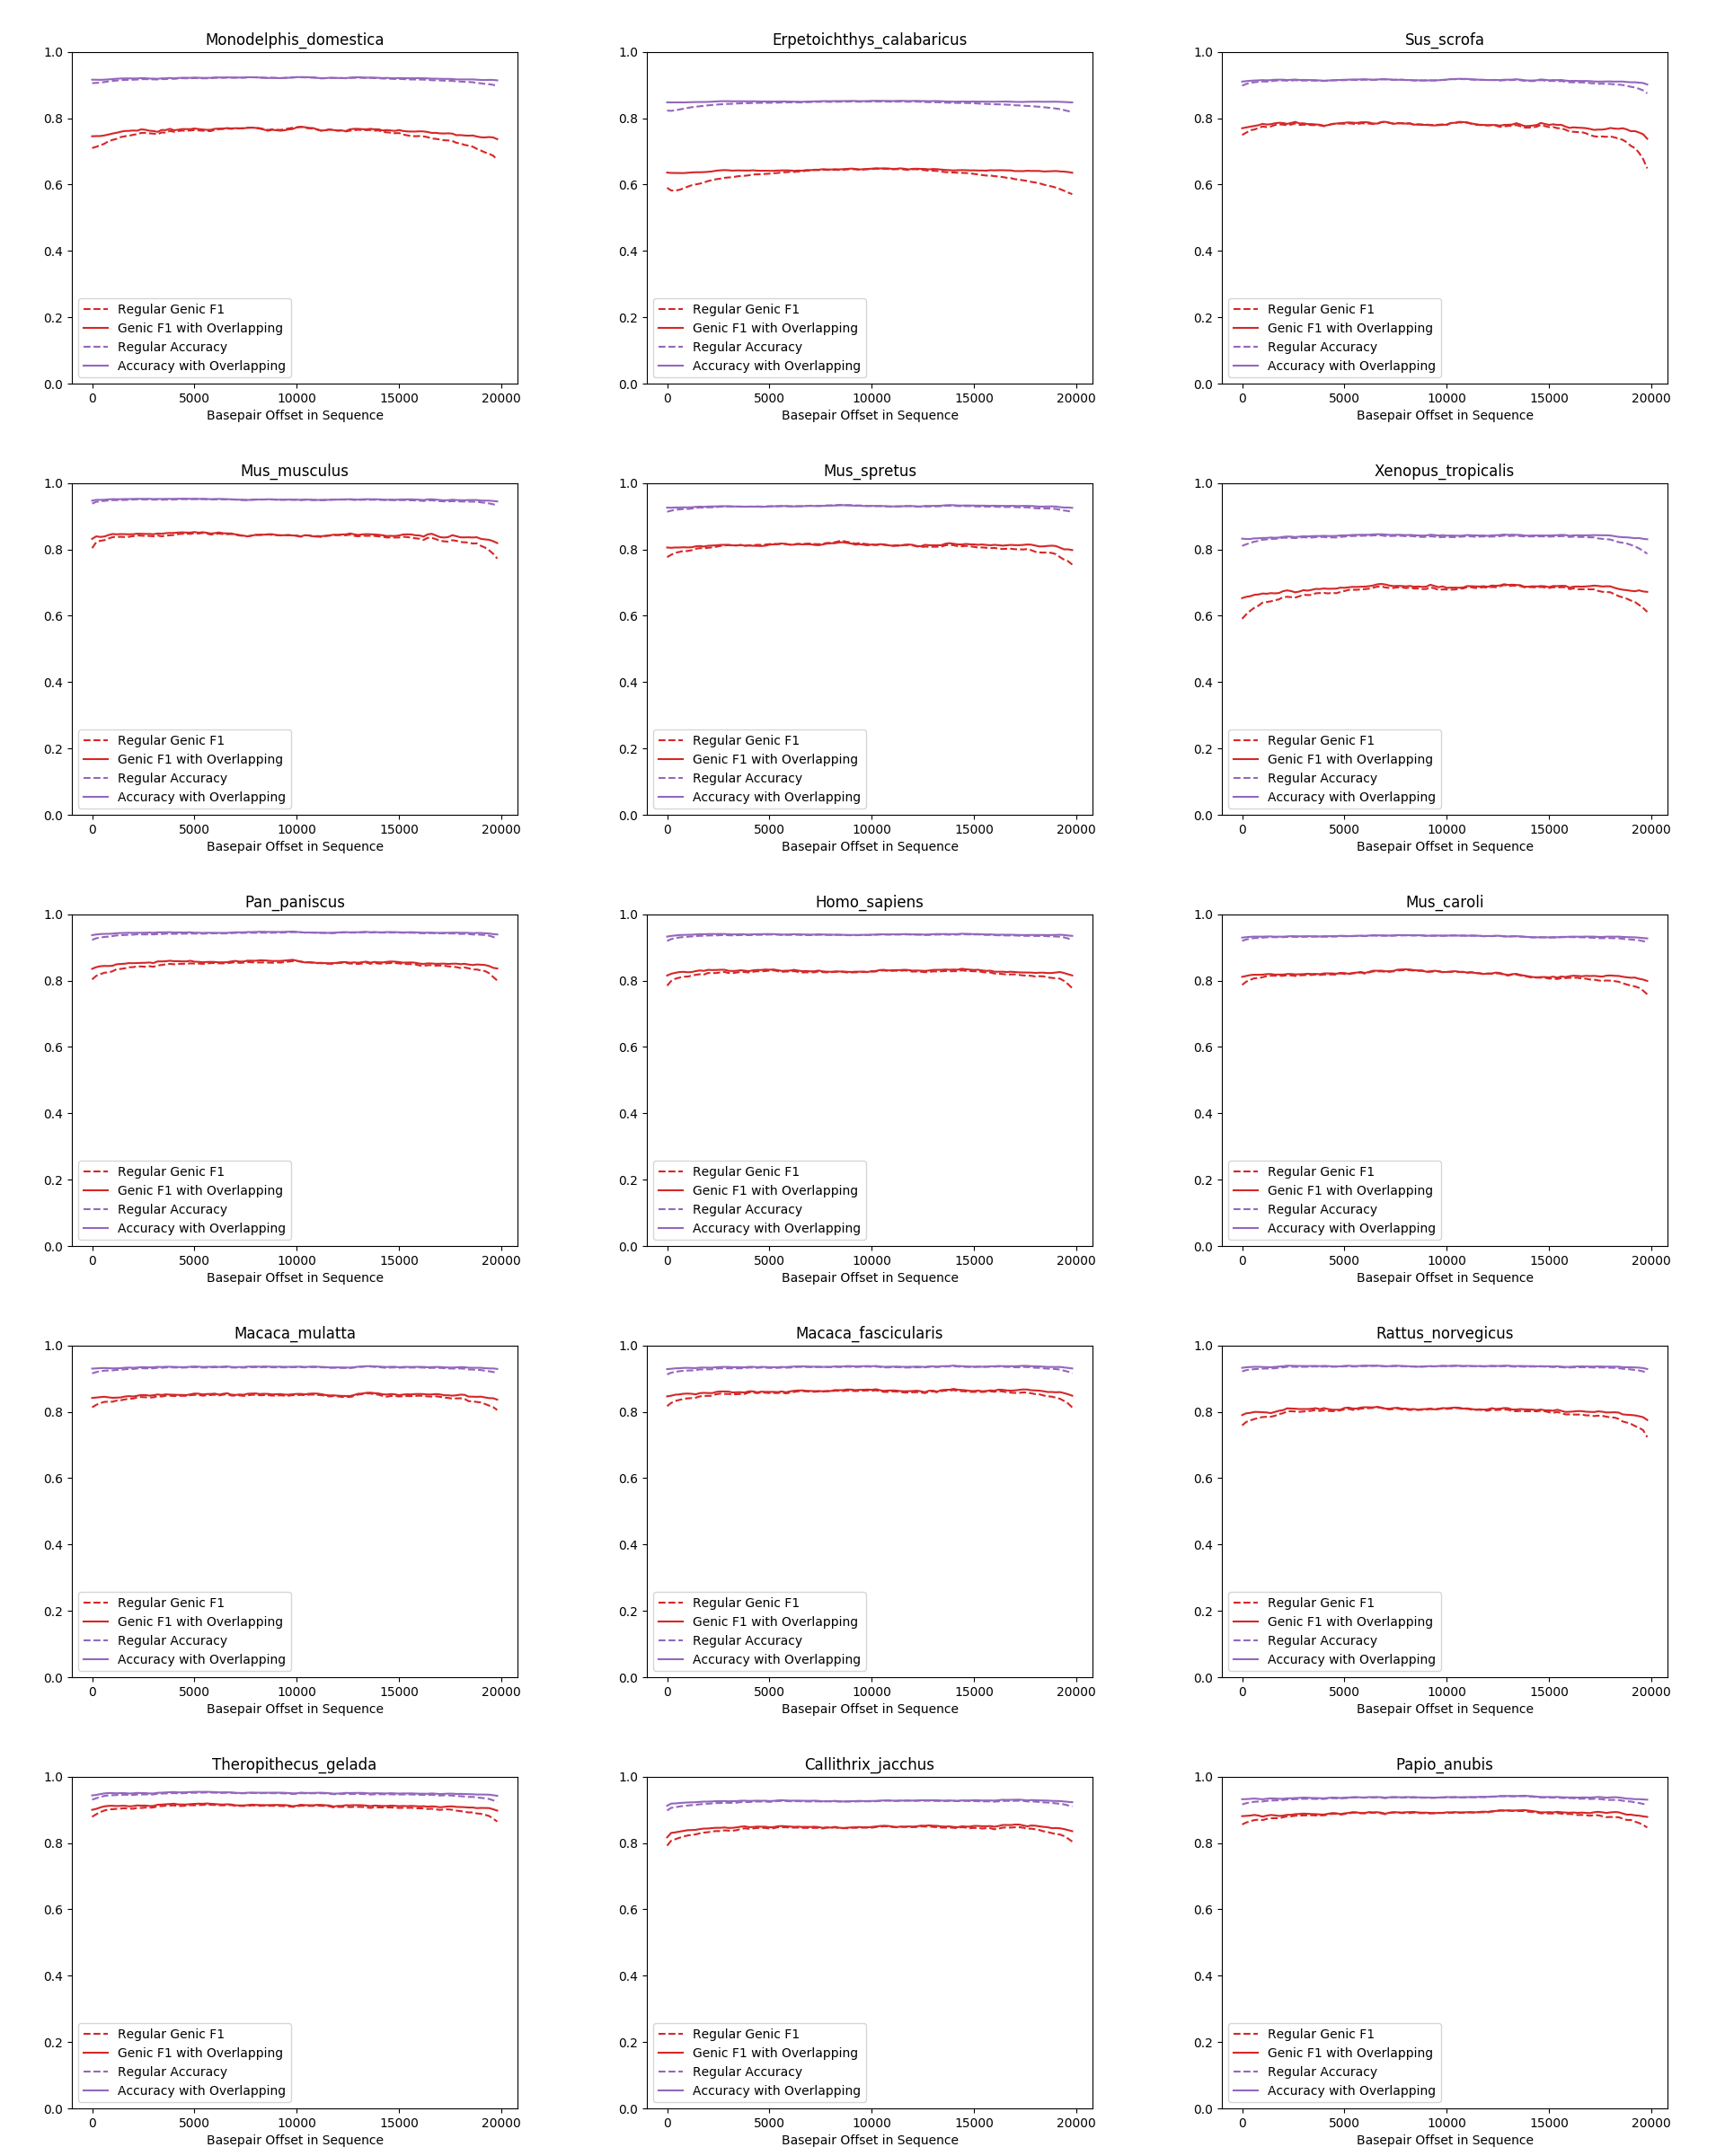
\includegraphics[width=1.2\textwidth]{images/overlapping/montage_animals1}}
\end{figure}
\begin{figure}[!h]
\centerline{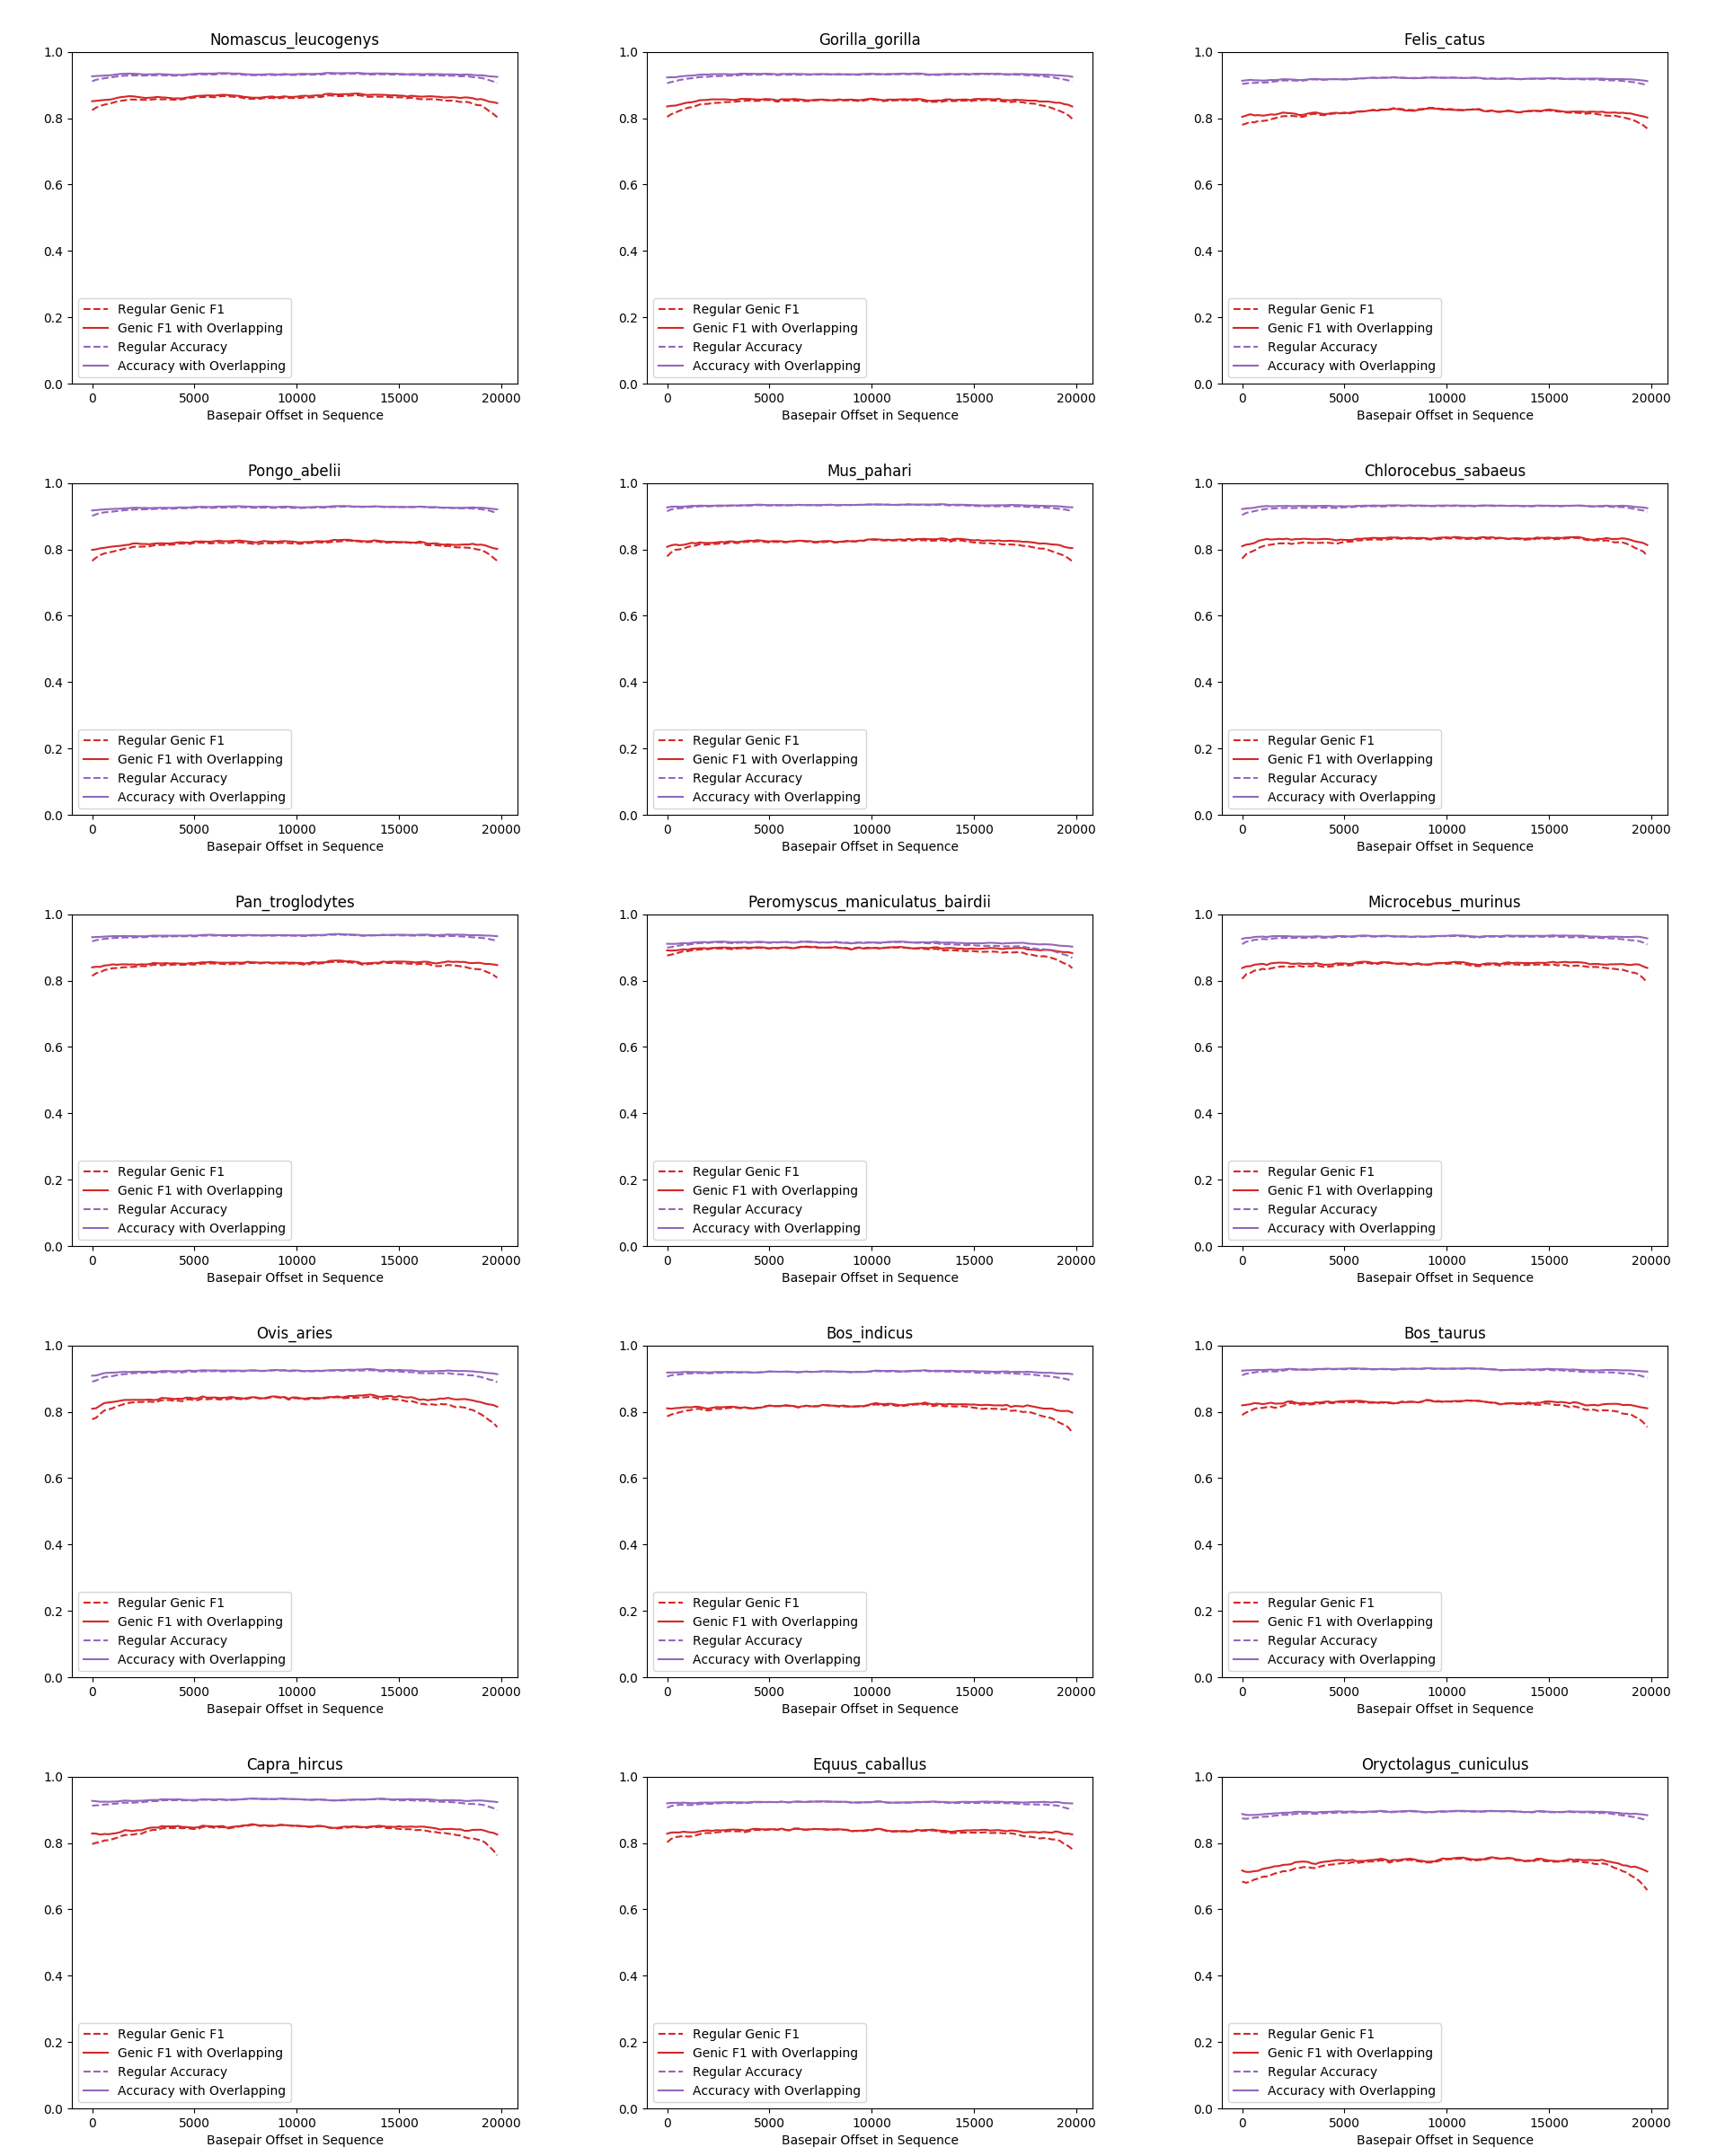
\includegraphics[width=1.2\textwidth]{images/overlapping/montage_animals2}}
\end{figure}
\begin{figure}[!h]
\centerline{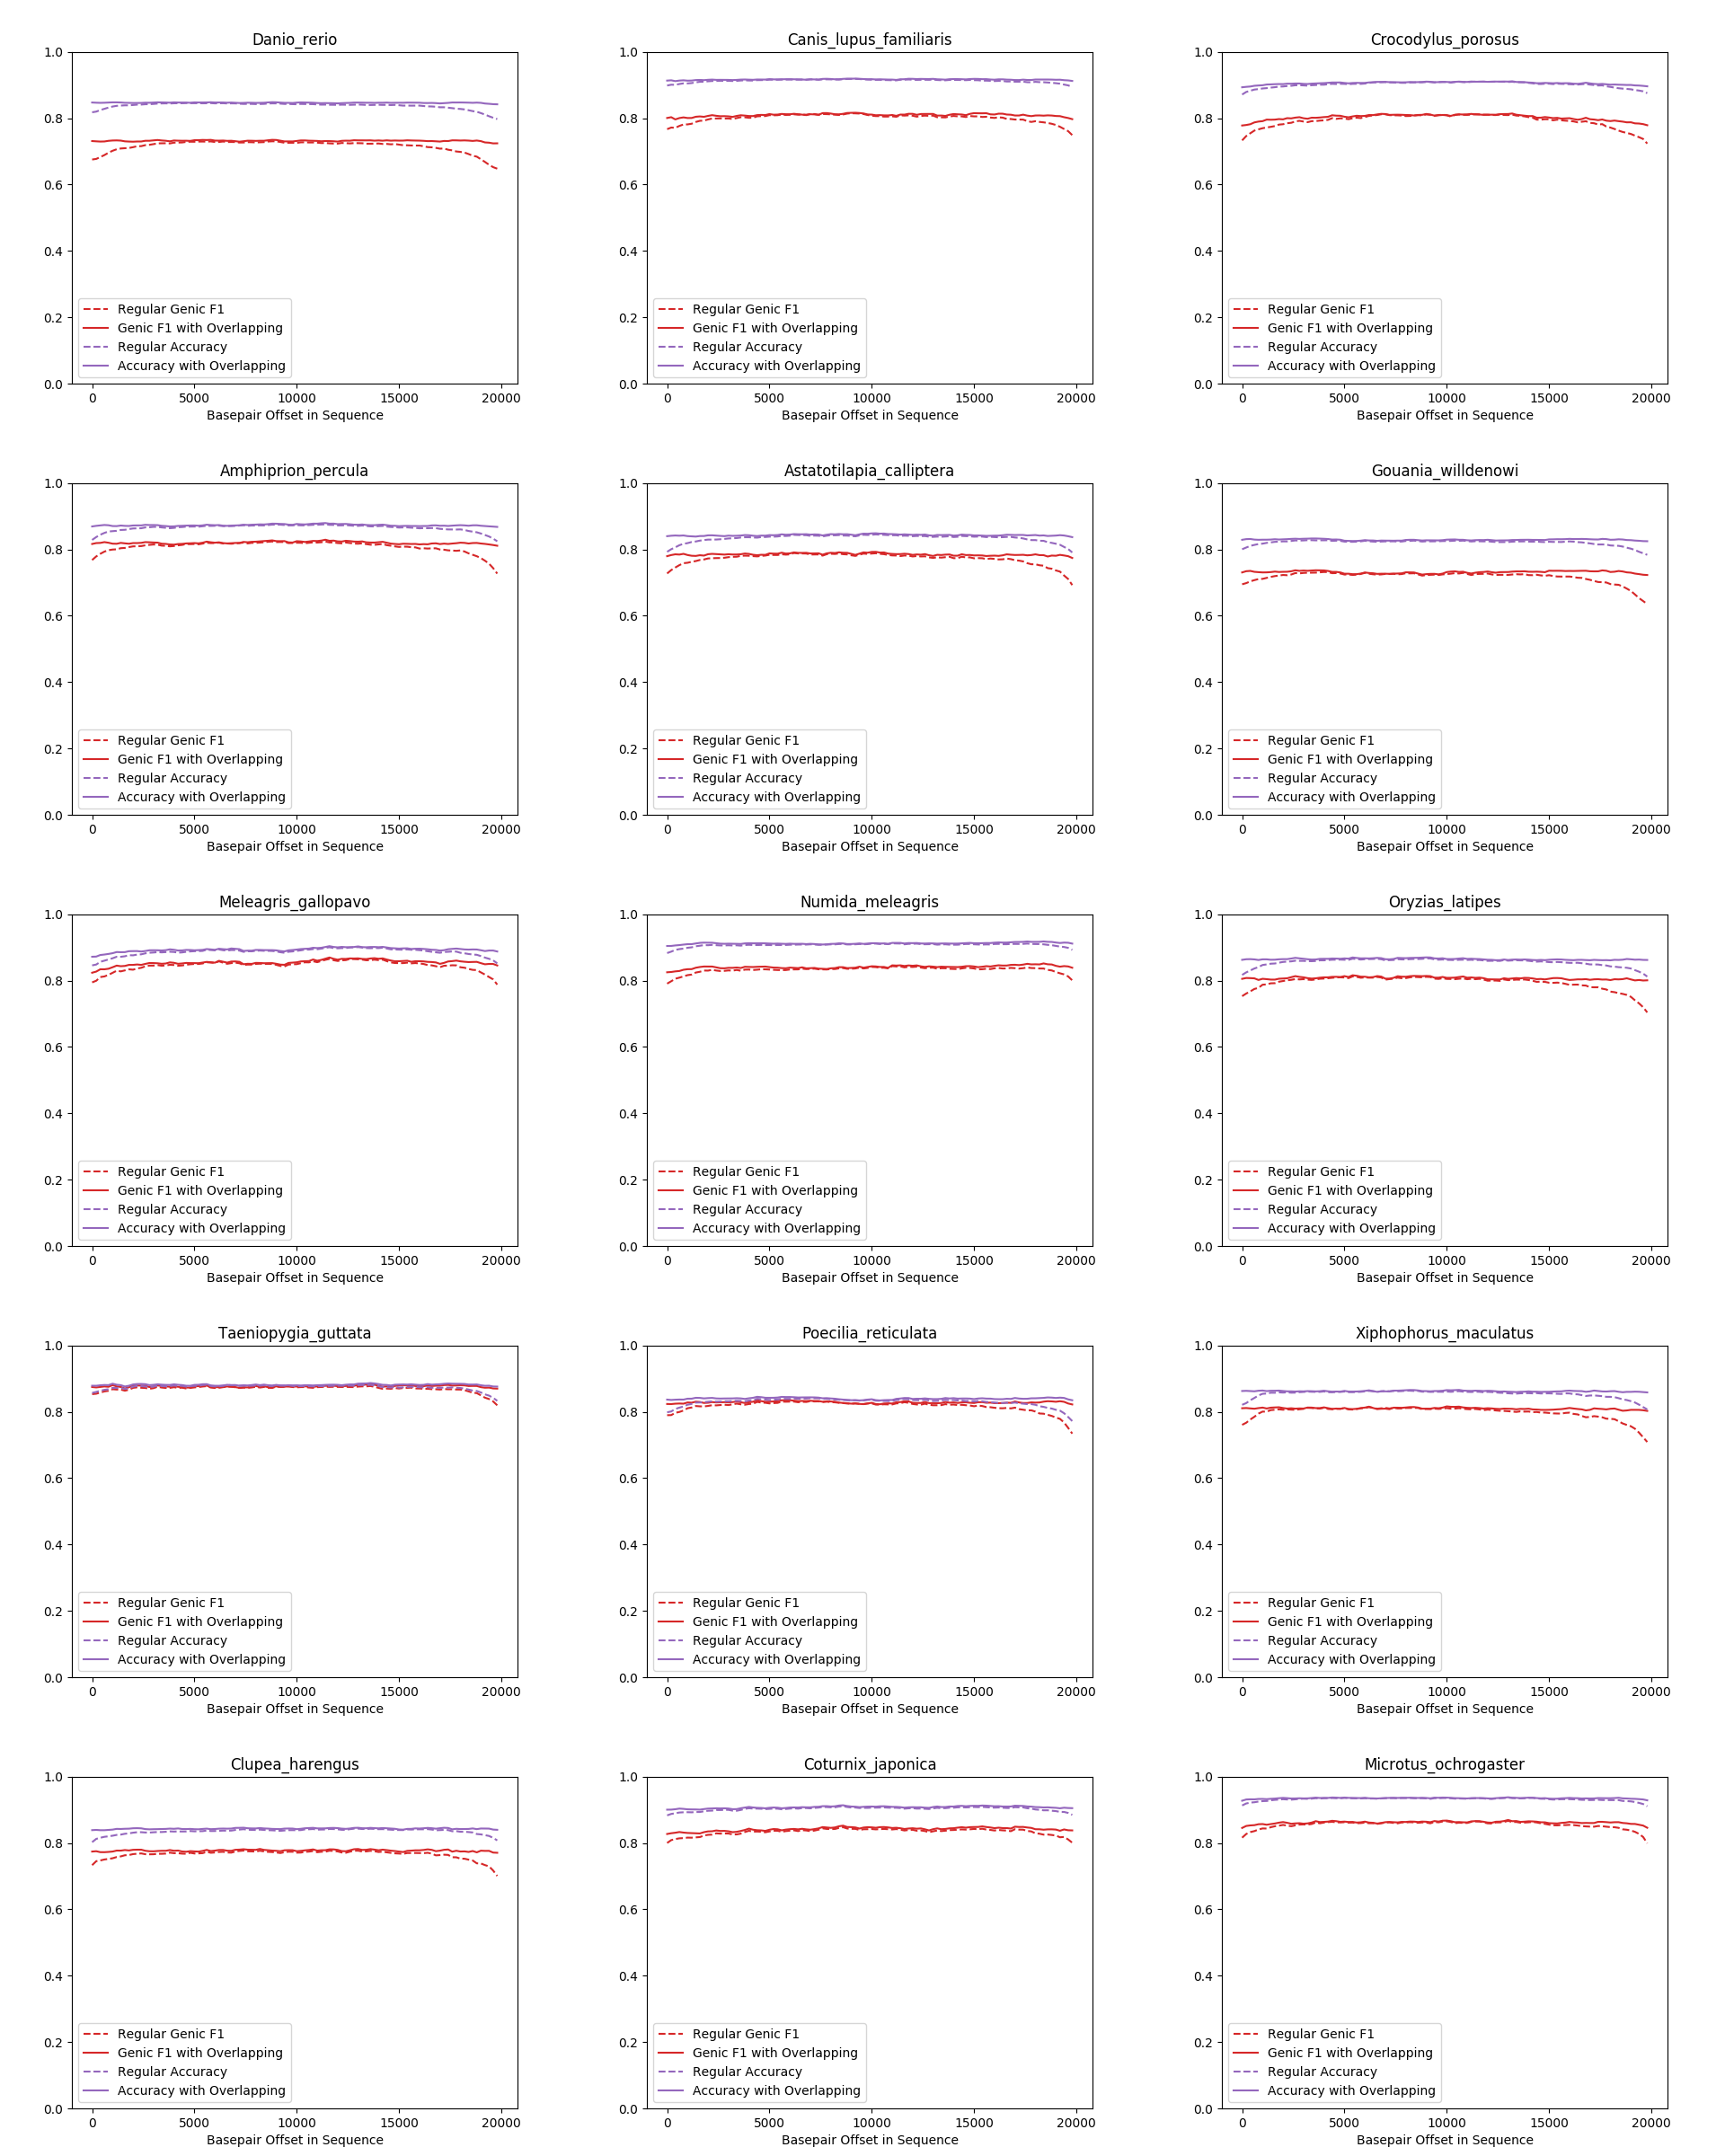
\includegraphics[width=1.2\textwidth]{images/overlapping/montage_animals3}}
\end{figure}
\begin{figure}[!h]
\centerline{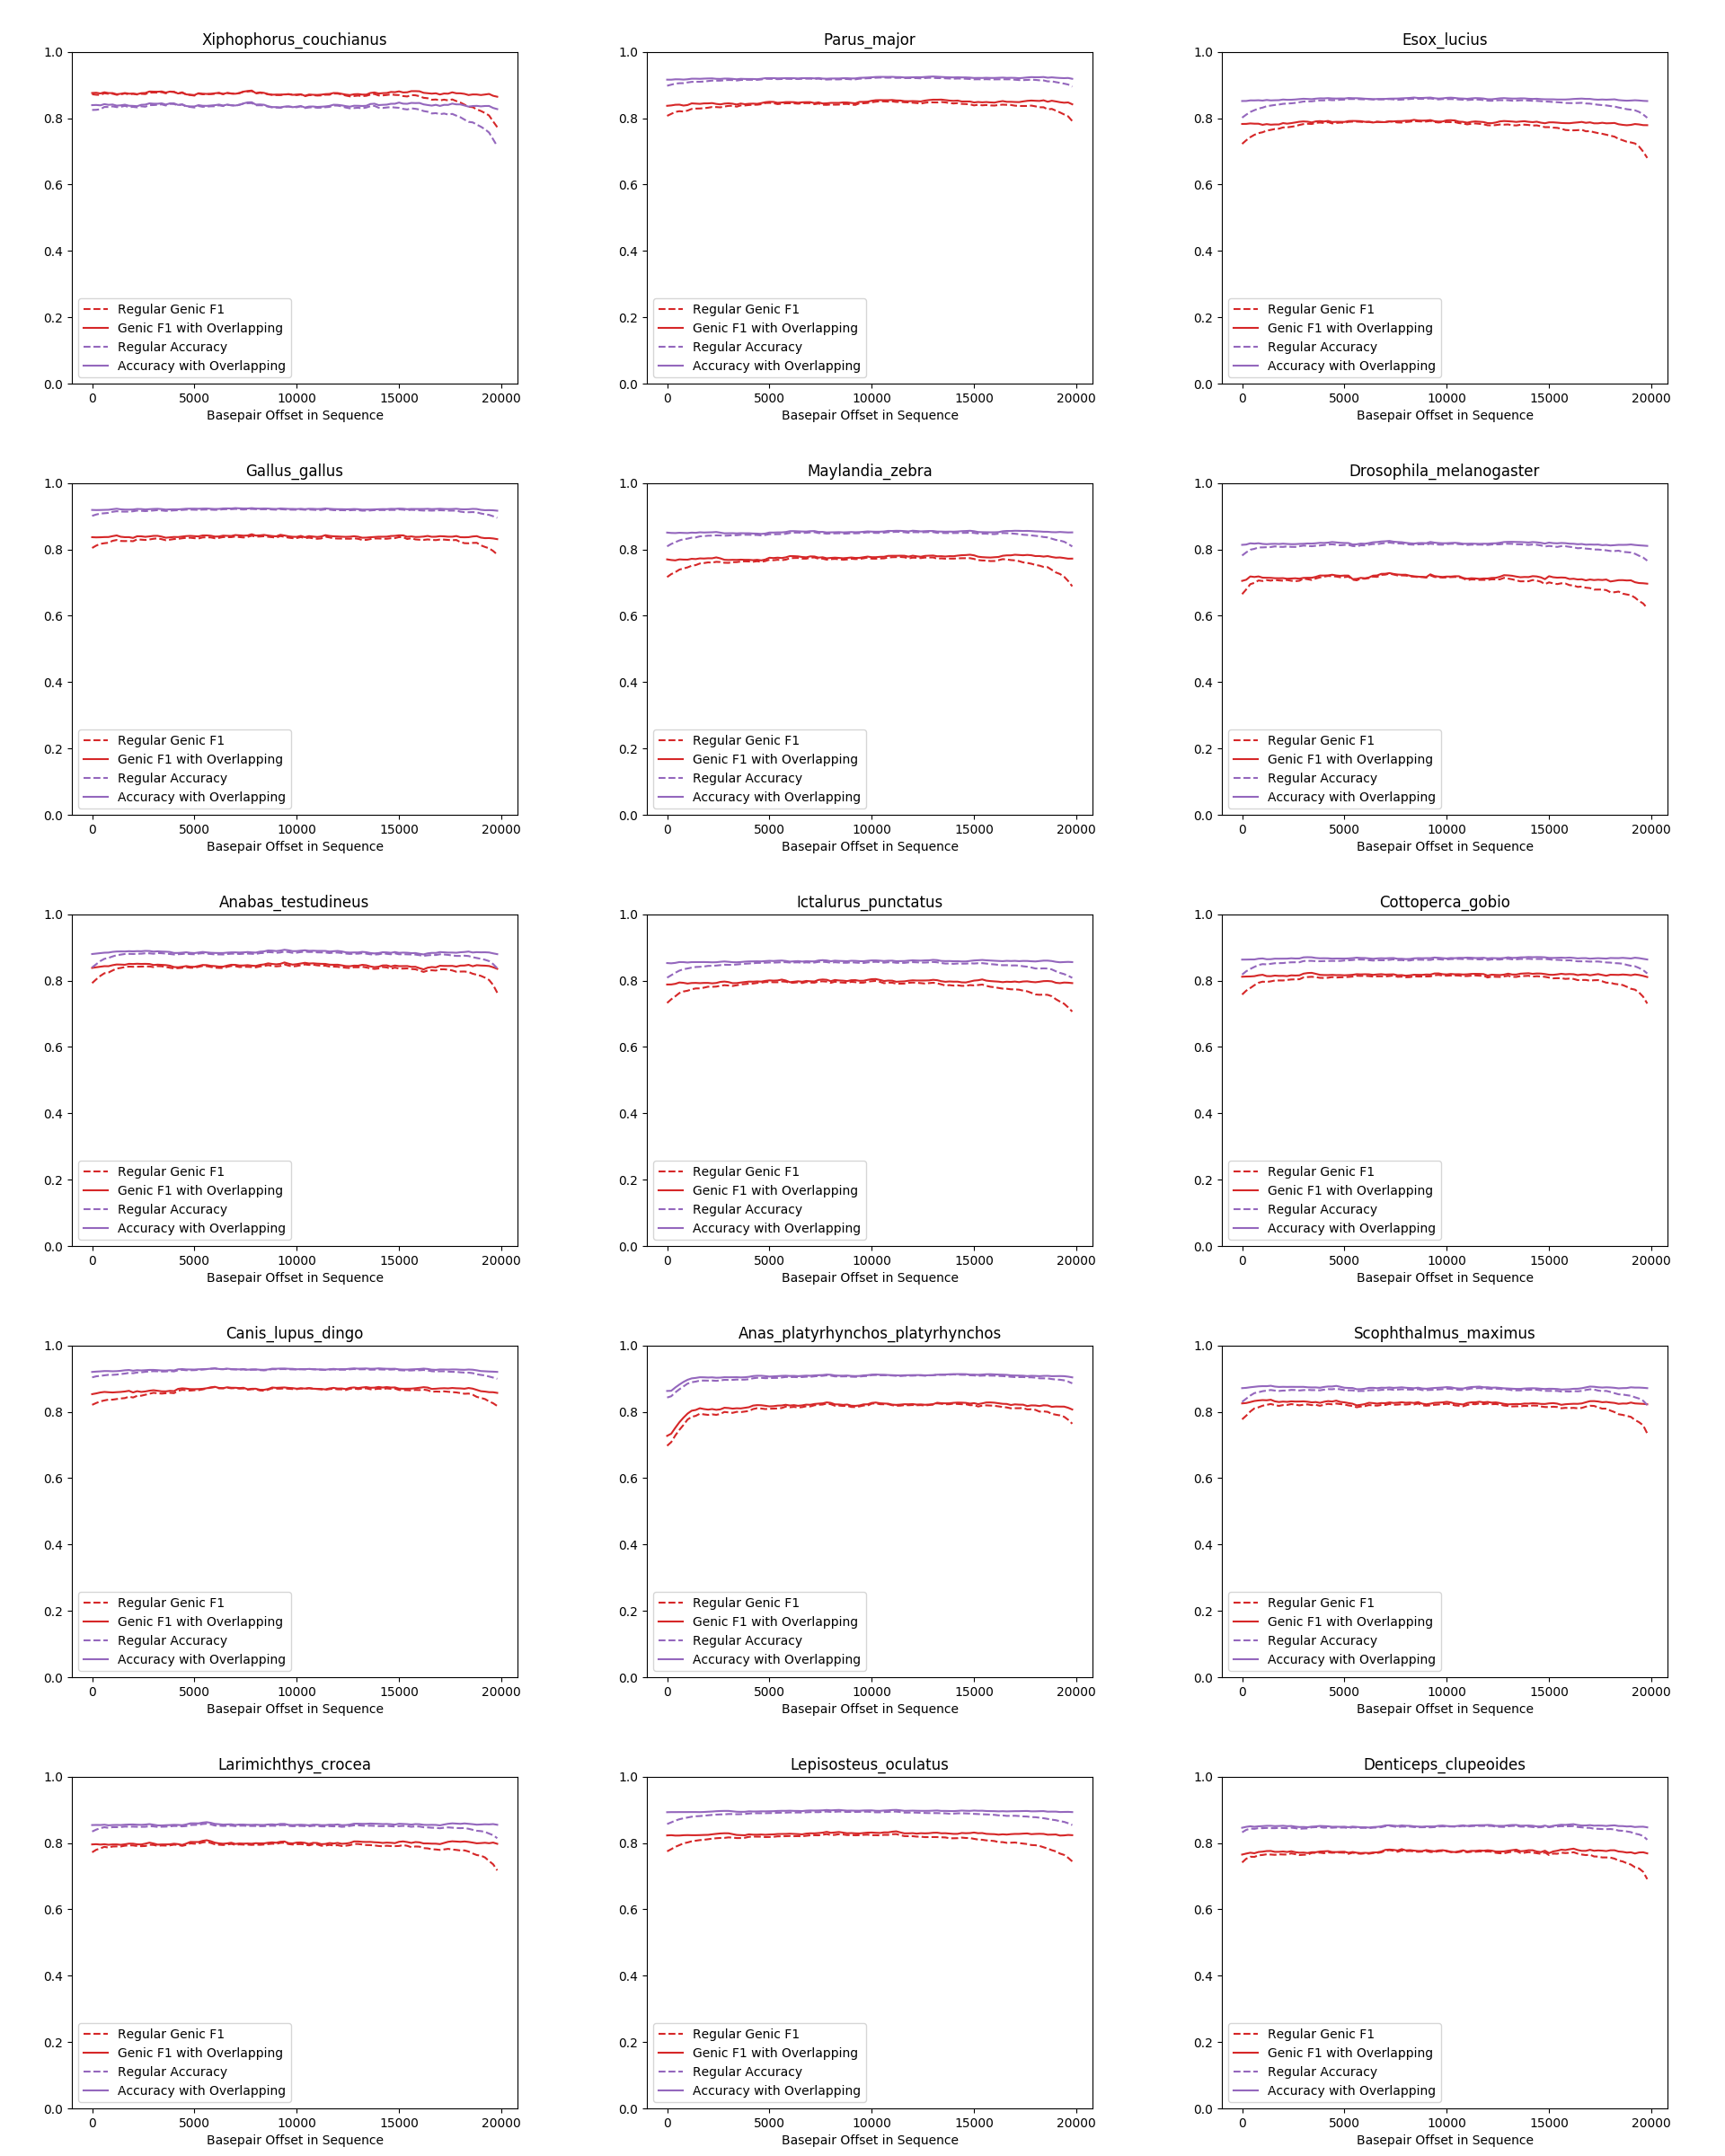
\includegraphics[width=1.2\textwidth]{images/overlapping/montage_animals4}}
\end{figure}
\begin{figure}[!h]
\centerline{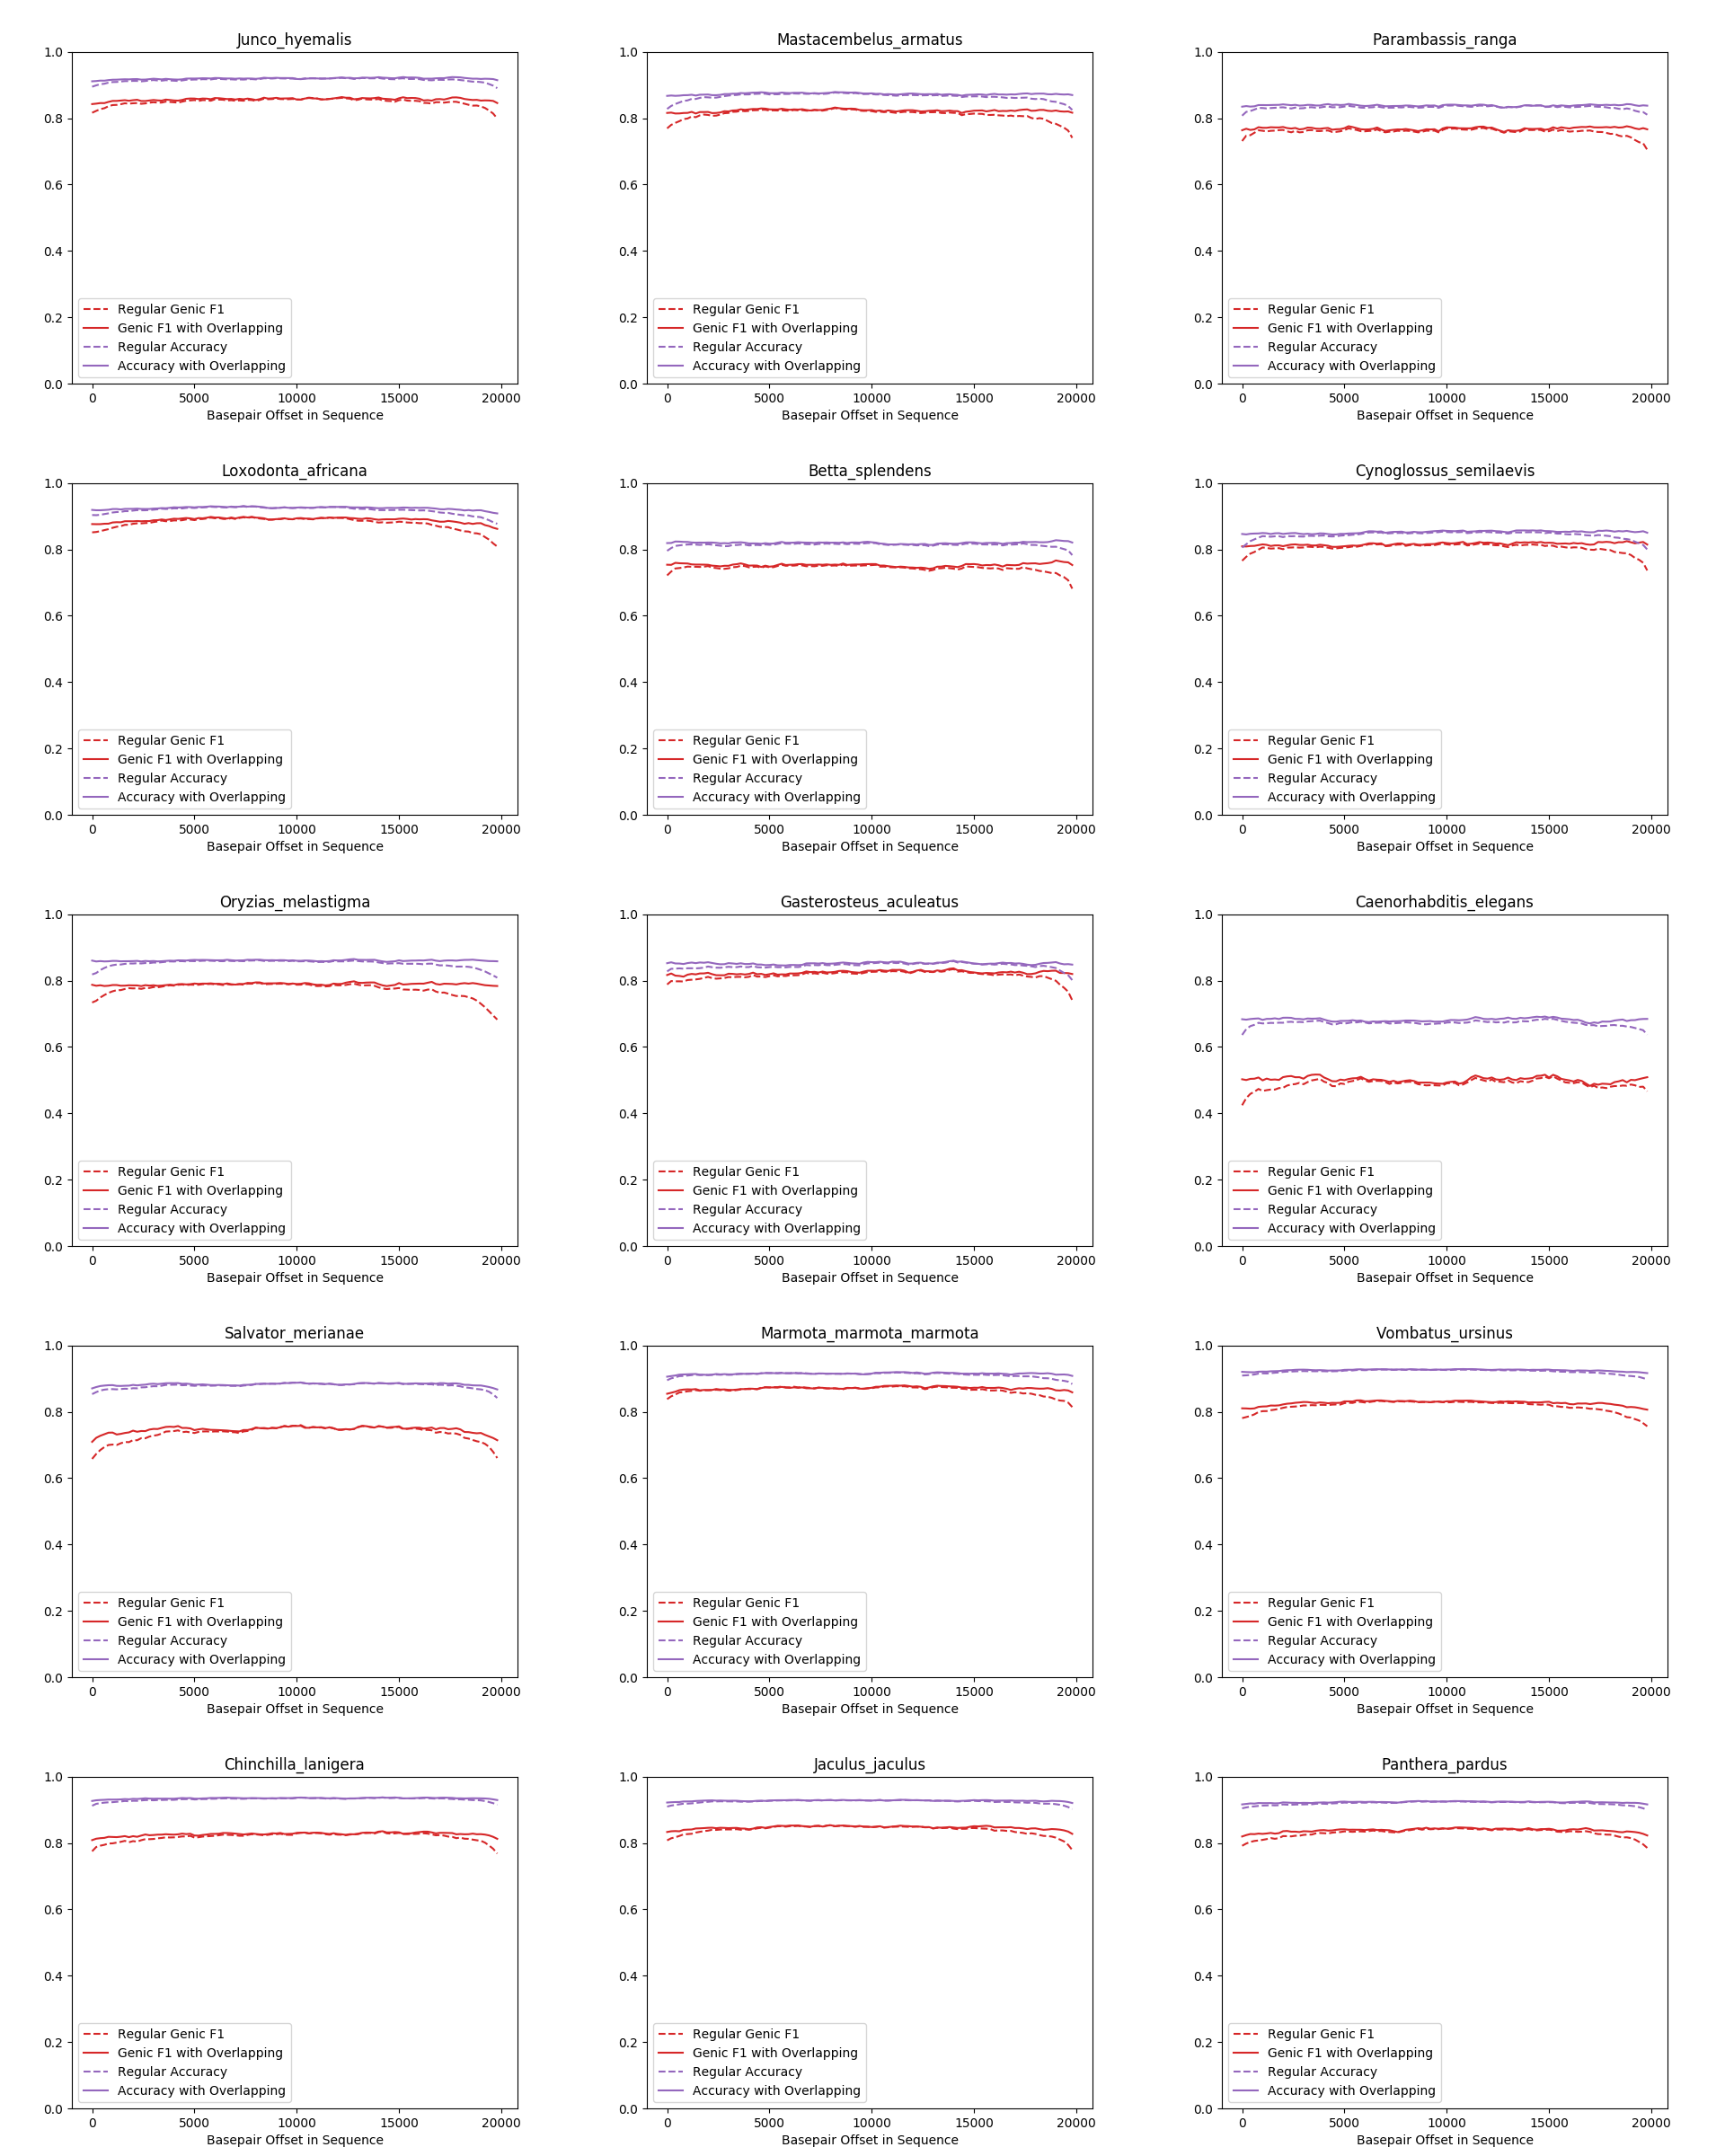
\includegraphics[width=1.2\textwidth]{images/overlapping/montage_animals5}}
\end{figure}
\begin{figure}[!h]
\centerline{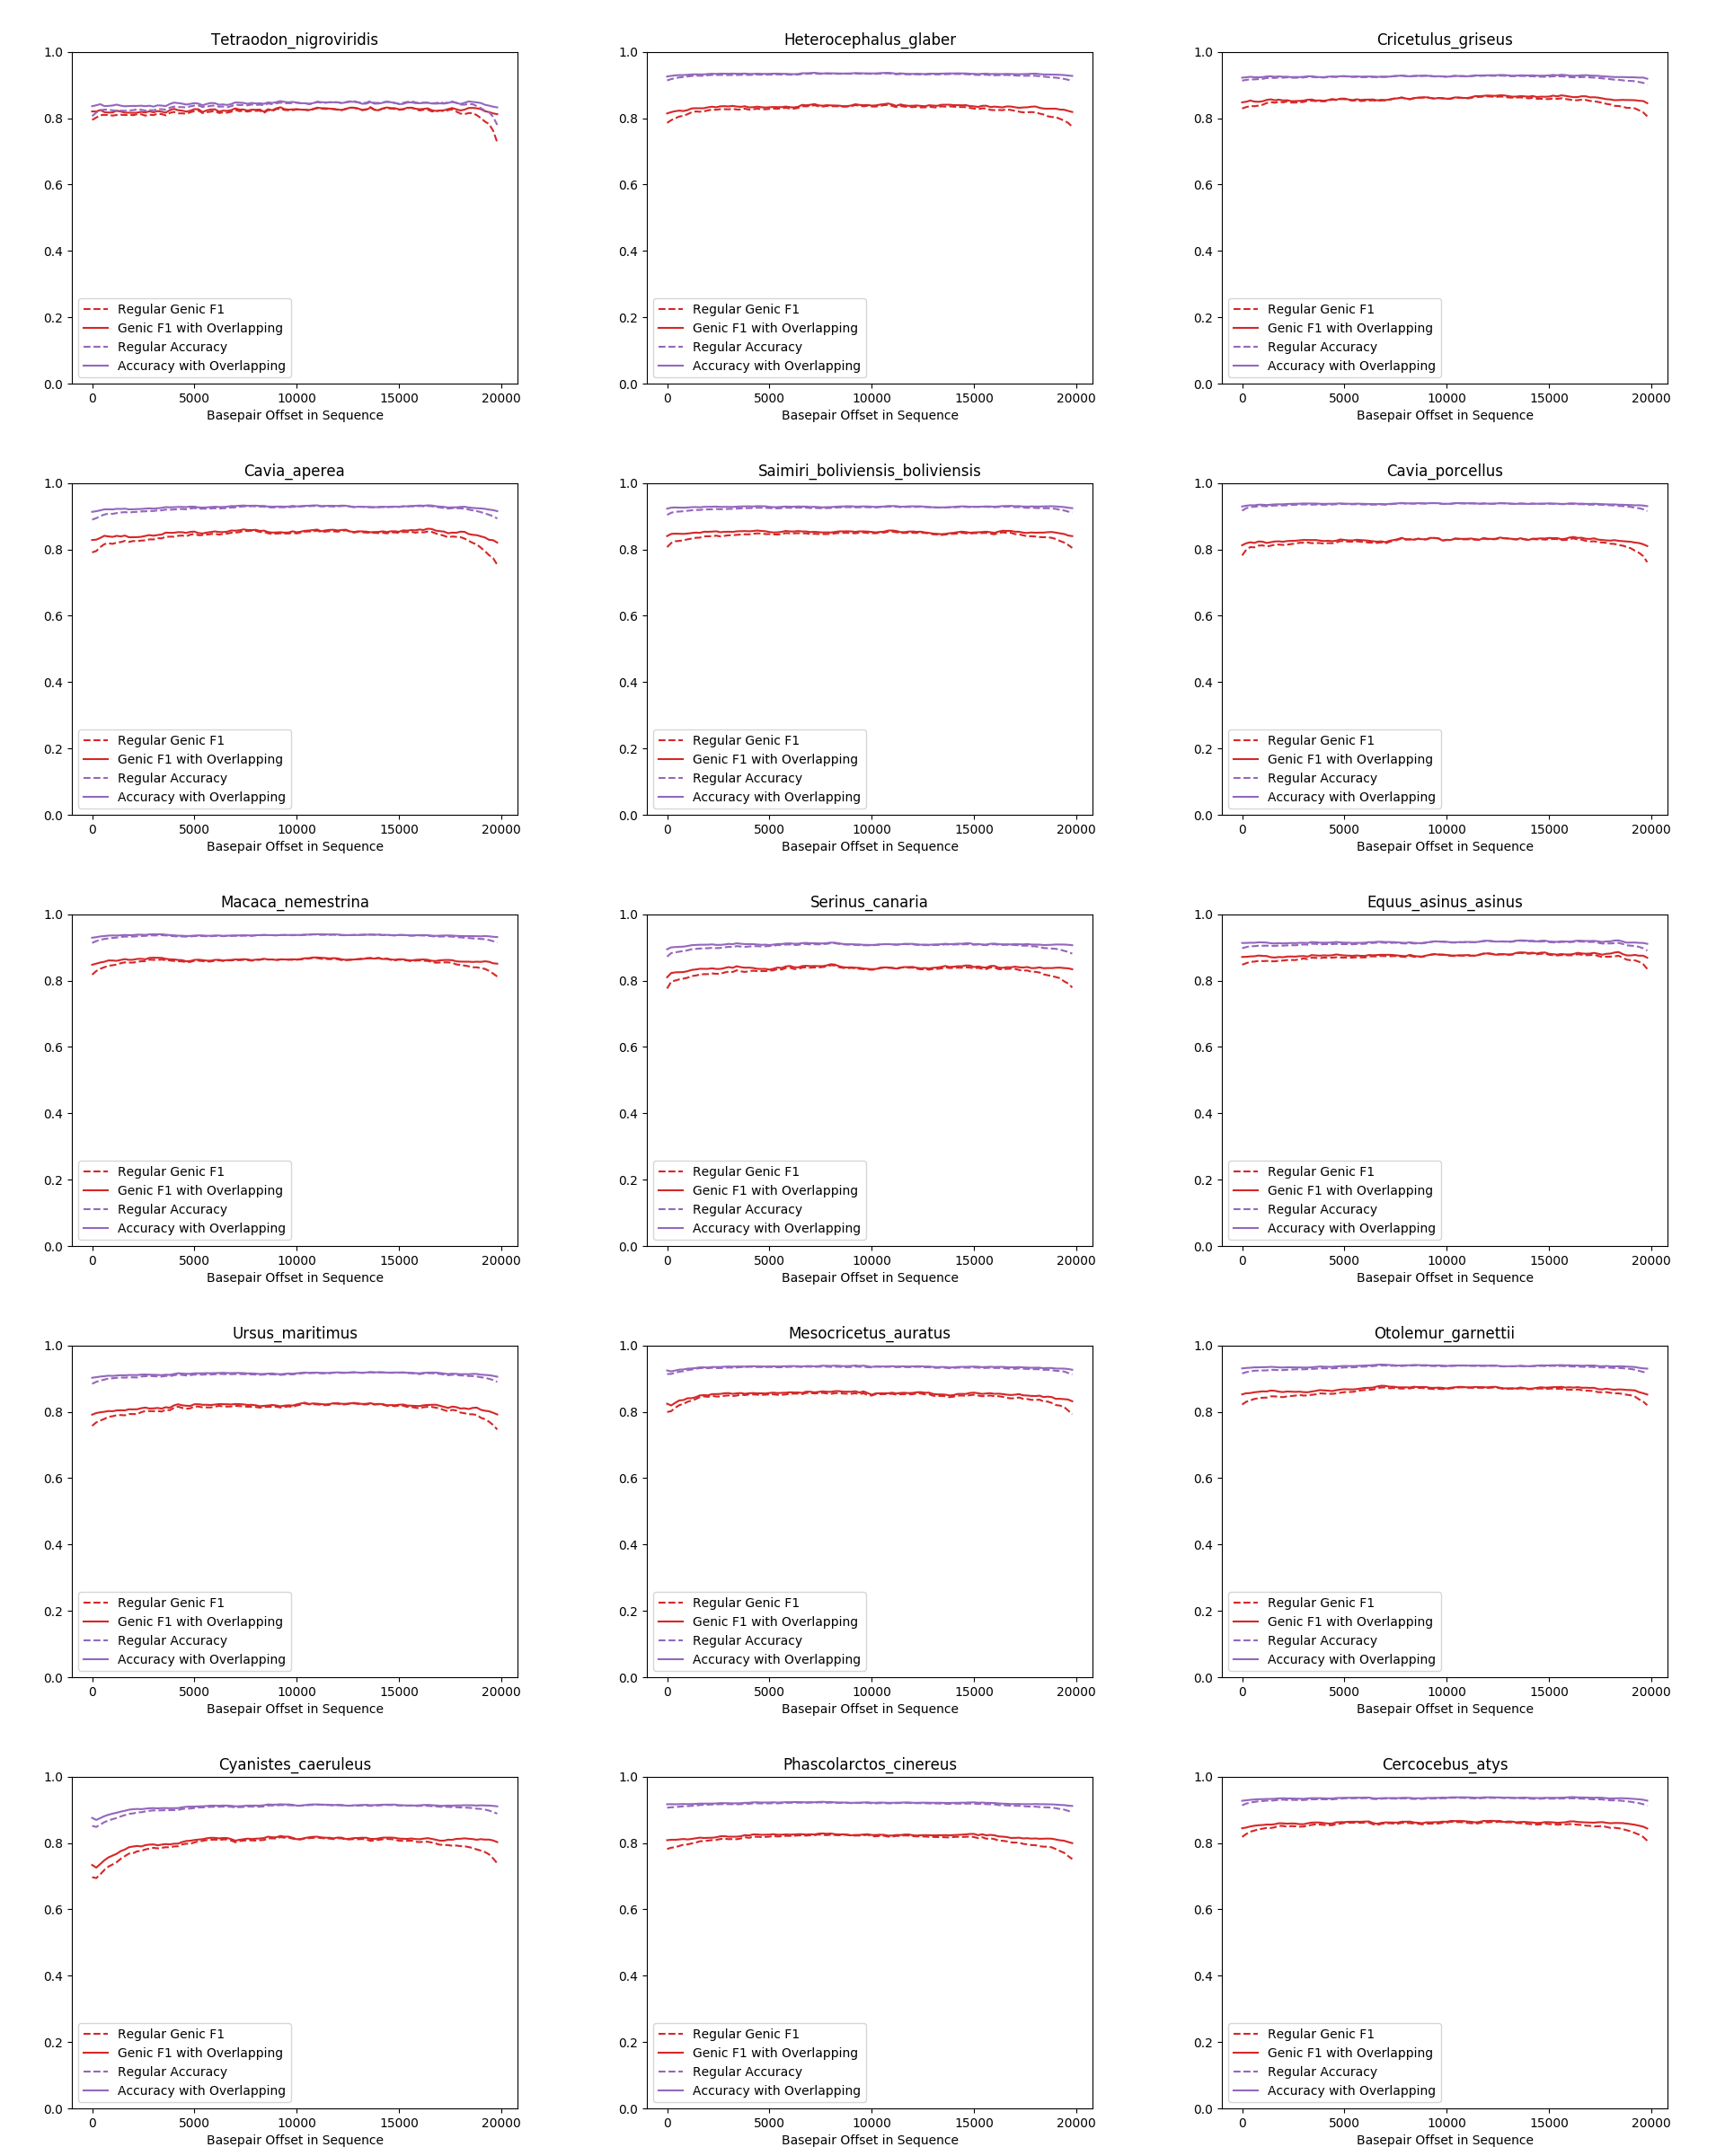
\includegraphics[width=1.2\textwidth]{images/overlapping/montage_animals6}}
\end{figure}
\begin{figure}[!h]
\centerline{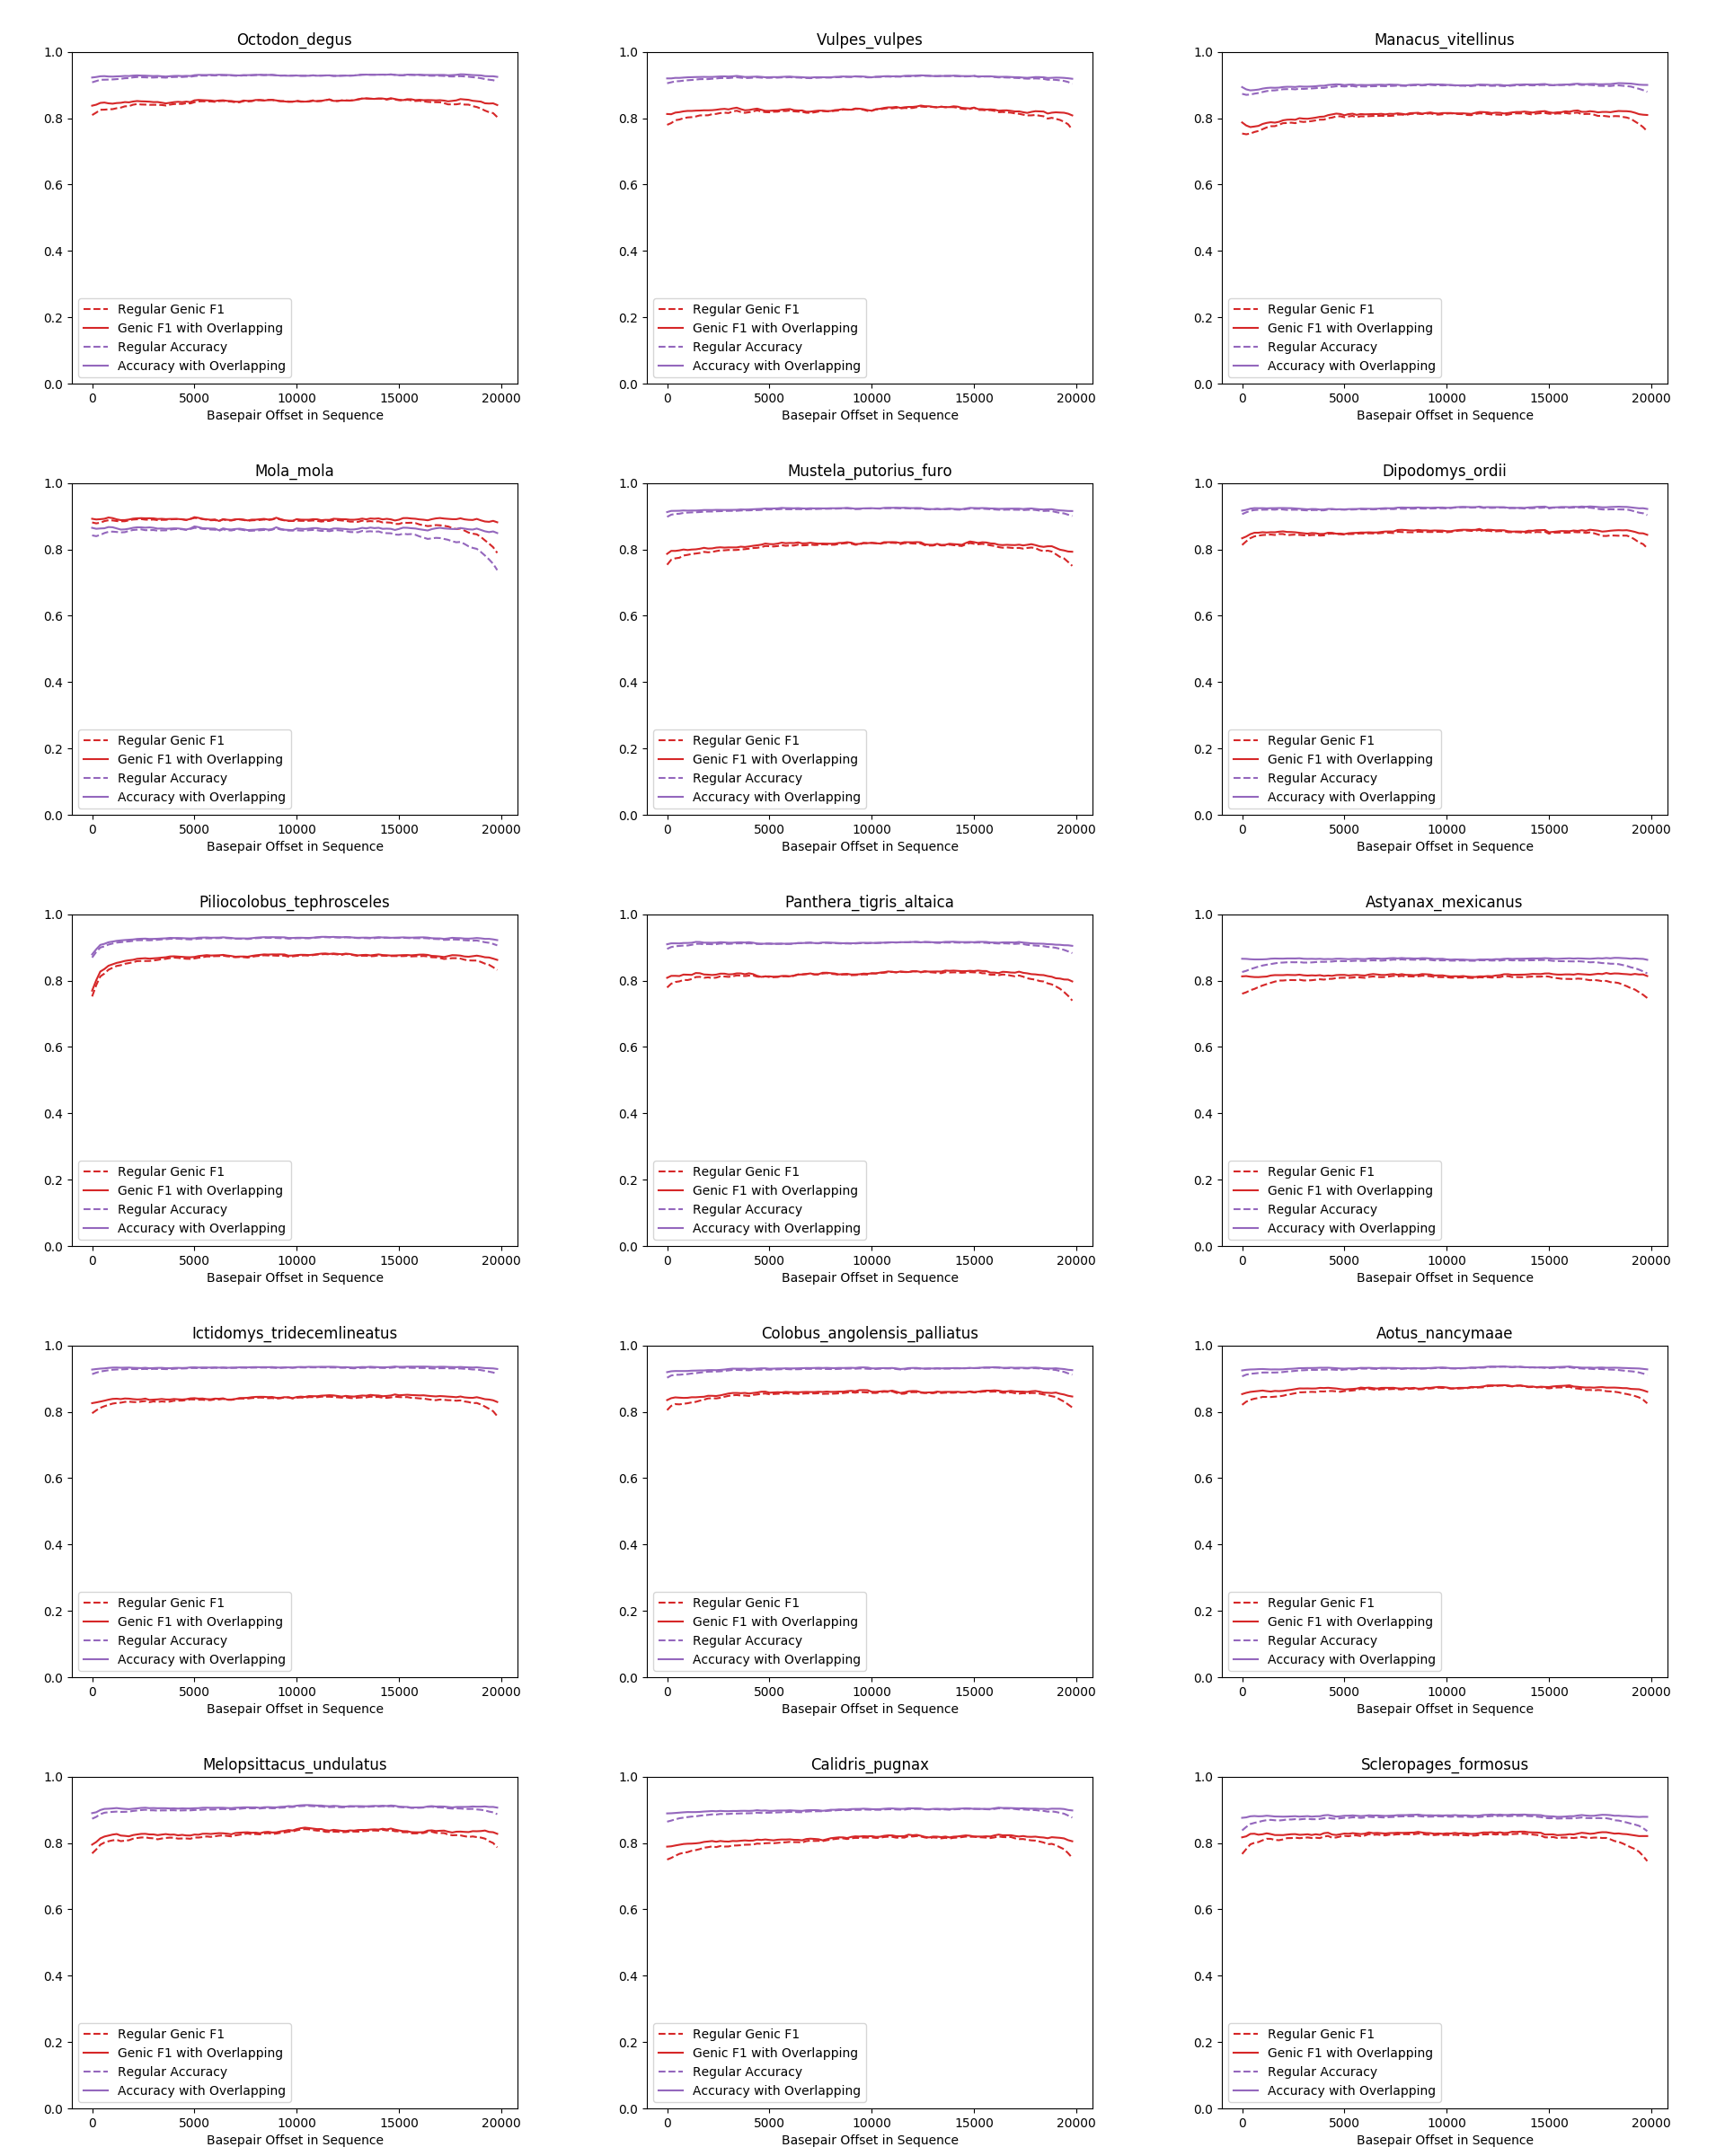
\includegraphics[width=1.2\textwidth]{images/overlapping/montage_animals7}}
\end{figure}
\begin{figure}[!h]
\centerline{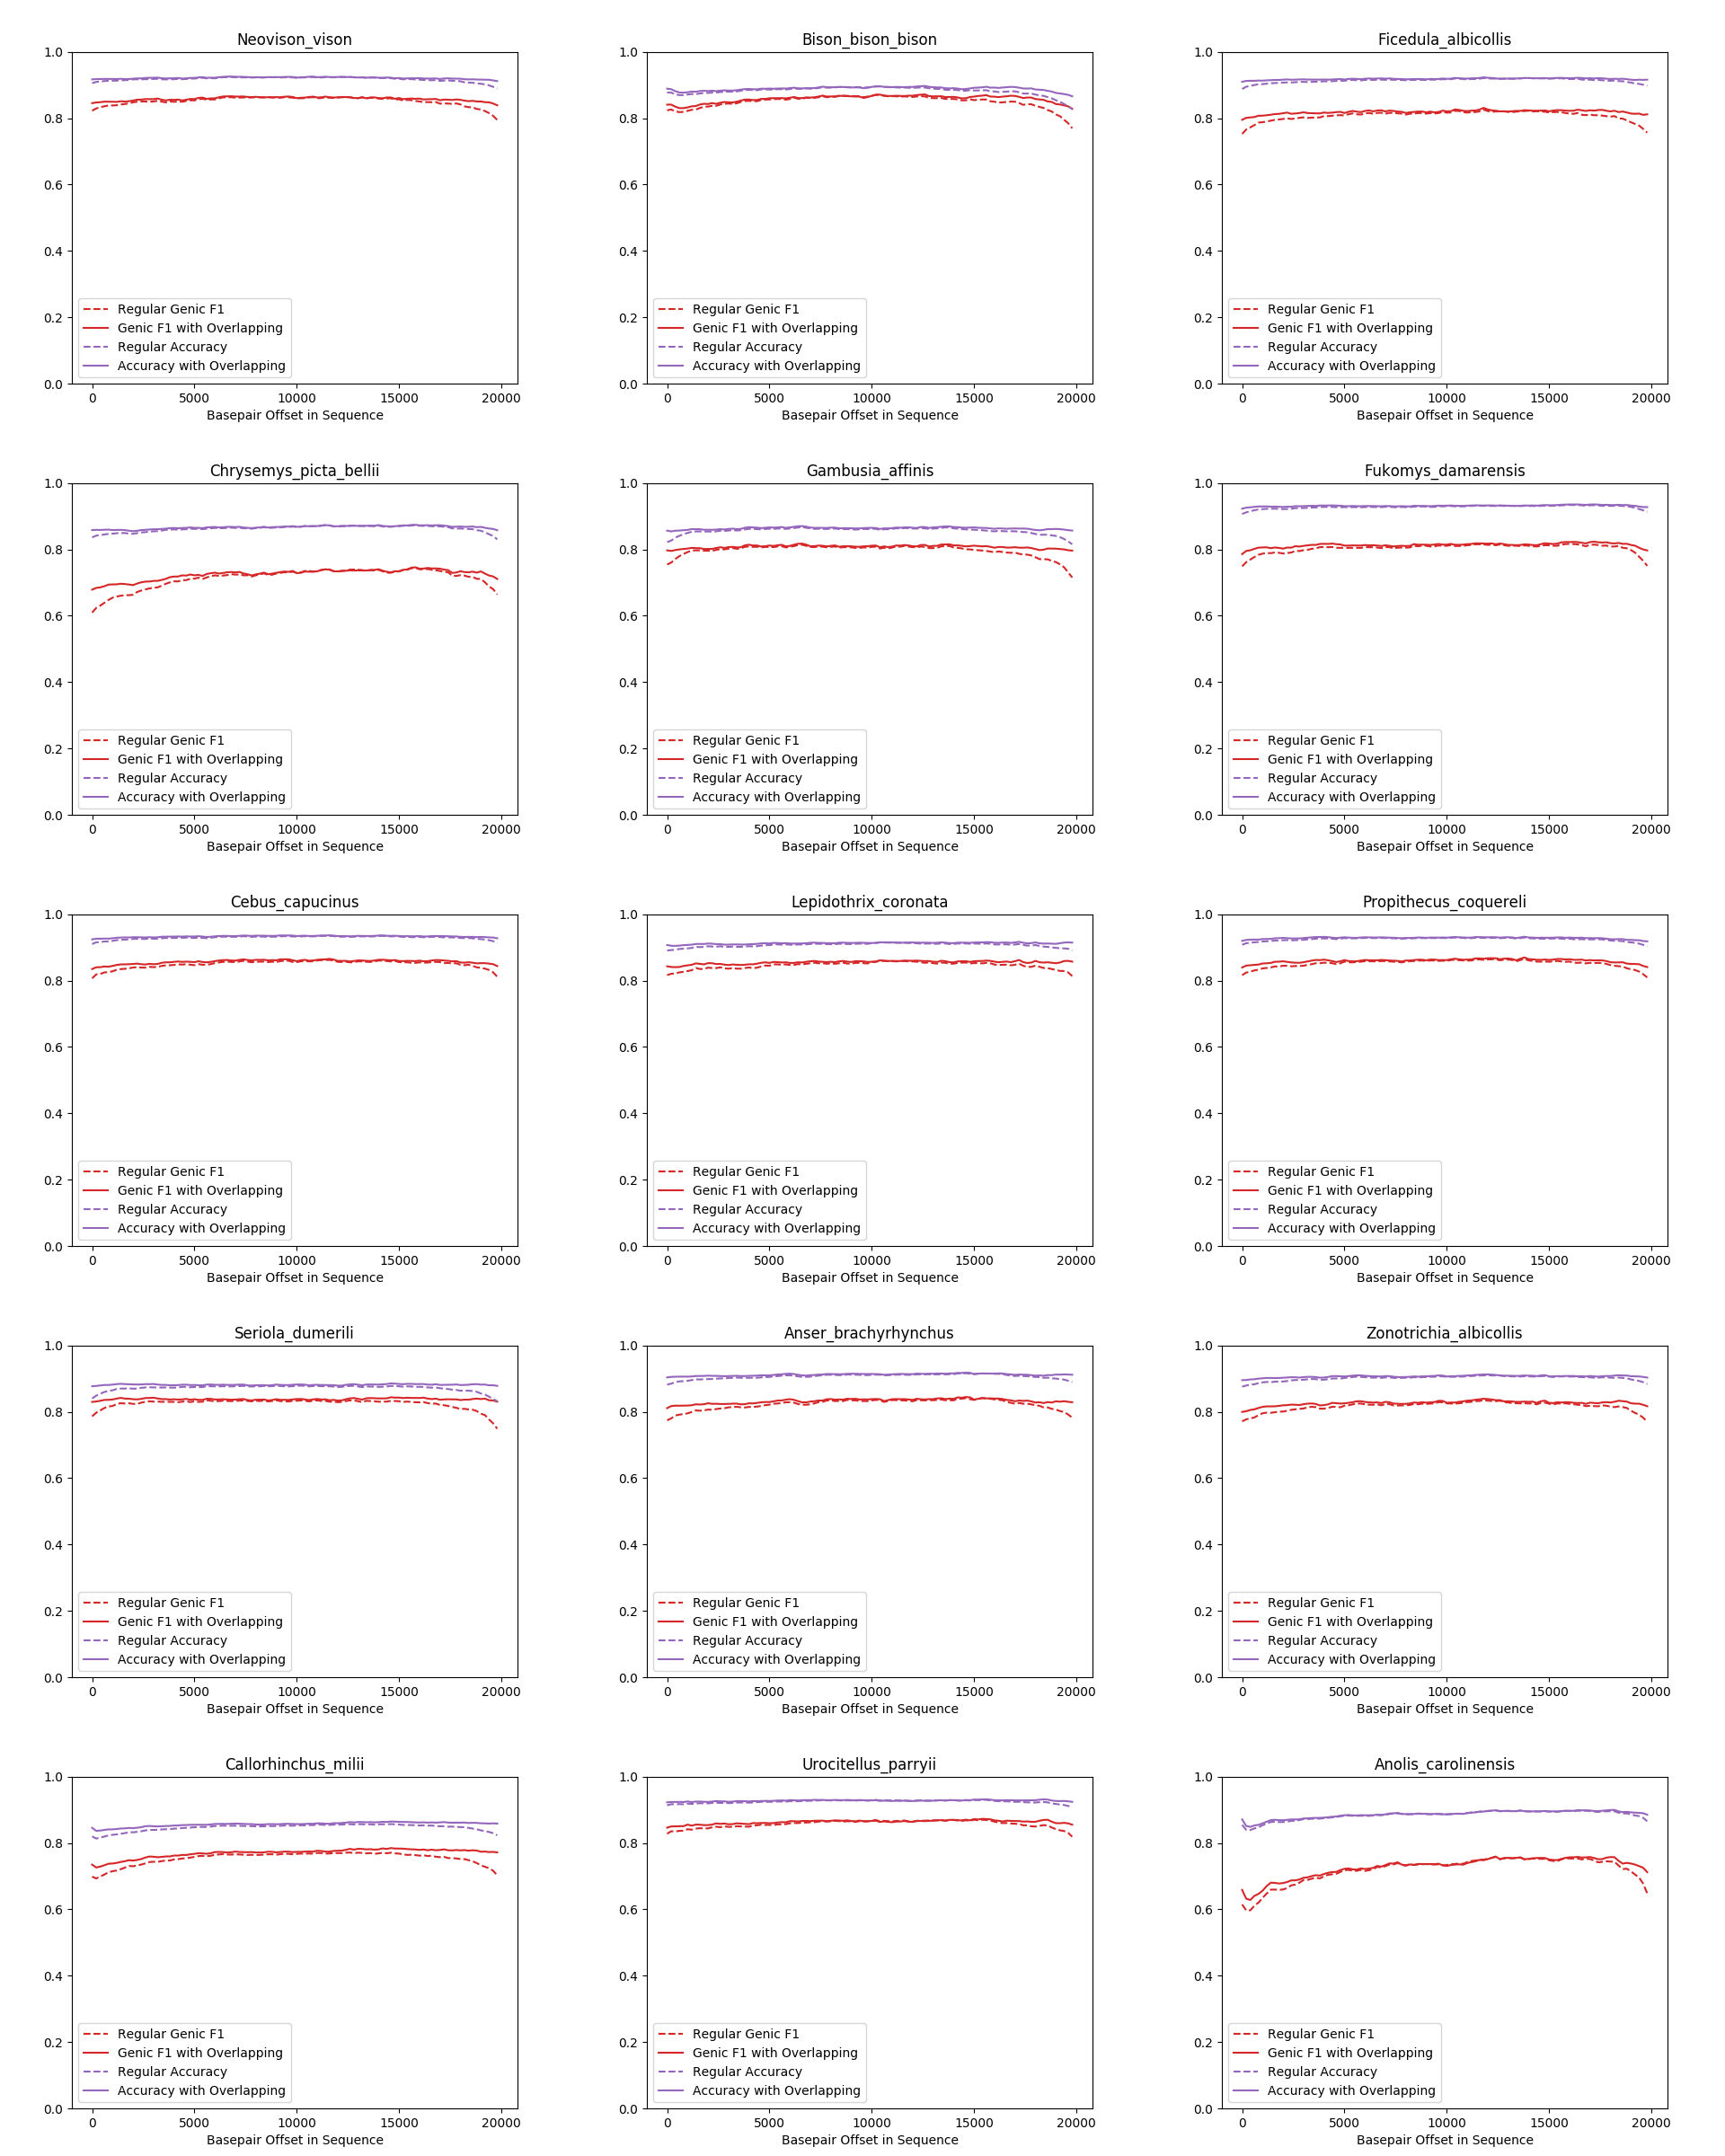
\includegraphics[width=1.2\textwidth]{images/overlapping/montage_animals8}}
\end{figure}
\begin{figure}[!h]
\centerline{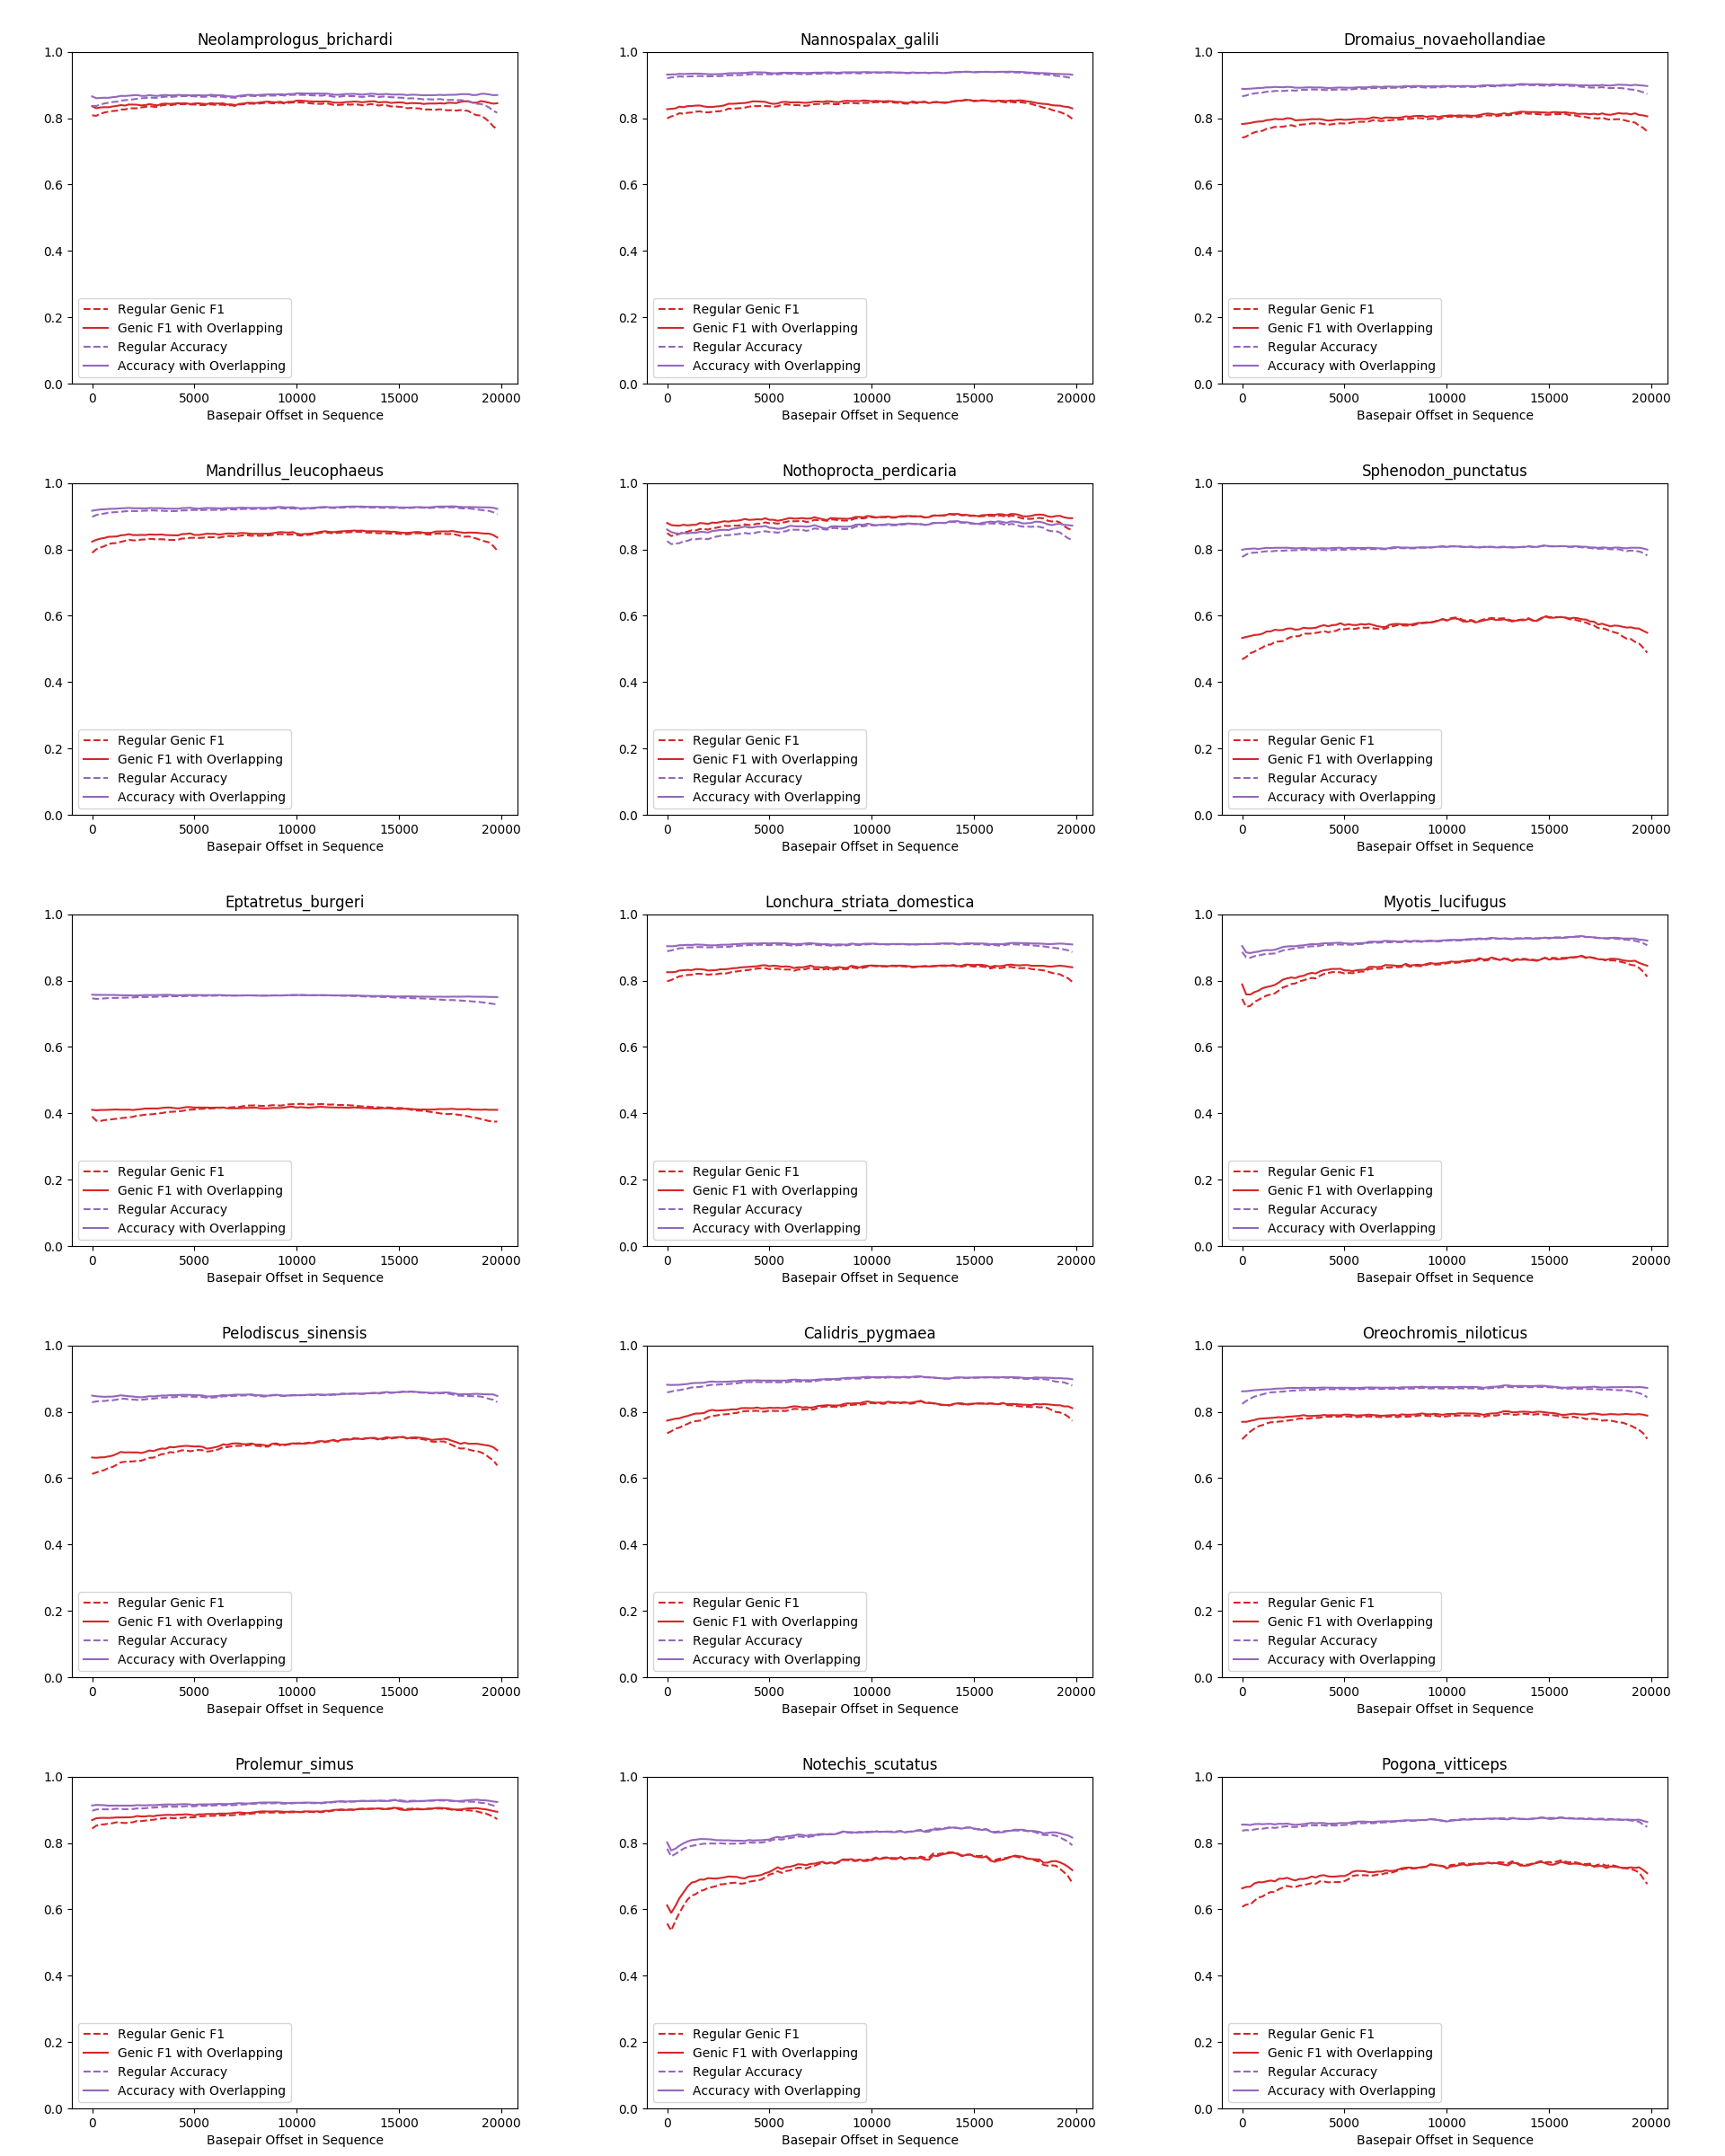
\includegraphics[width=1.2\textwidth]{images/overlapping/montage_animals9}}
\end{figure}
\begin{figure}[!h]
\centerline{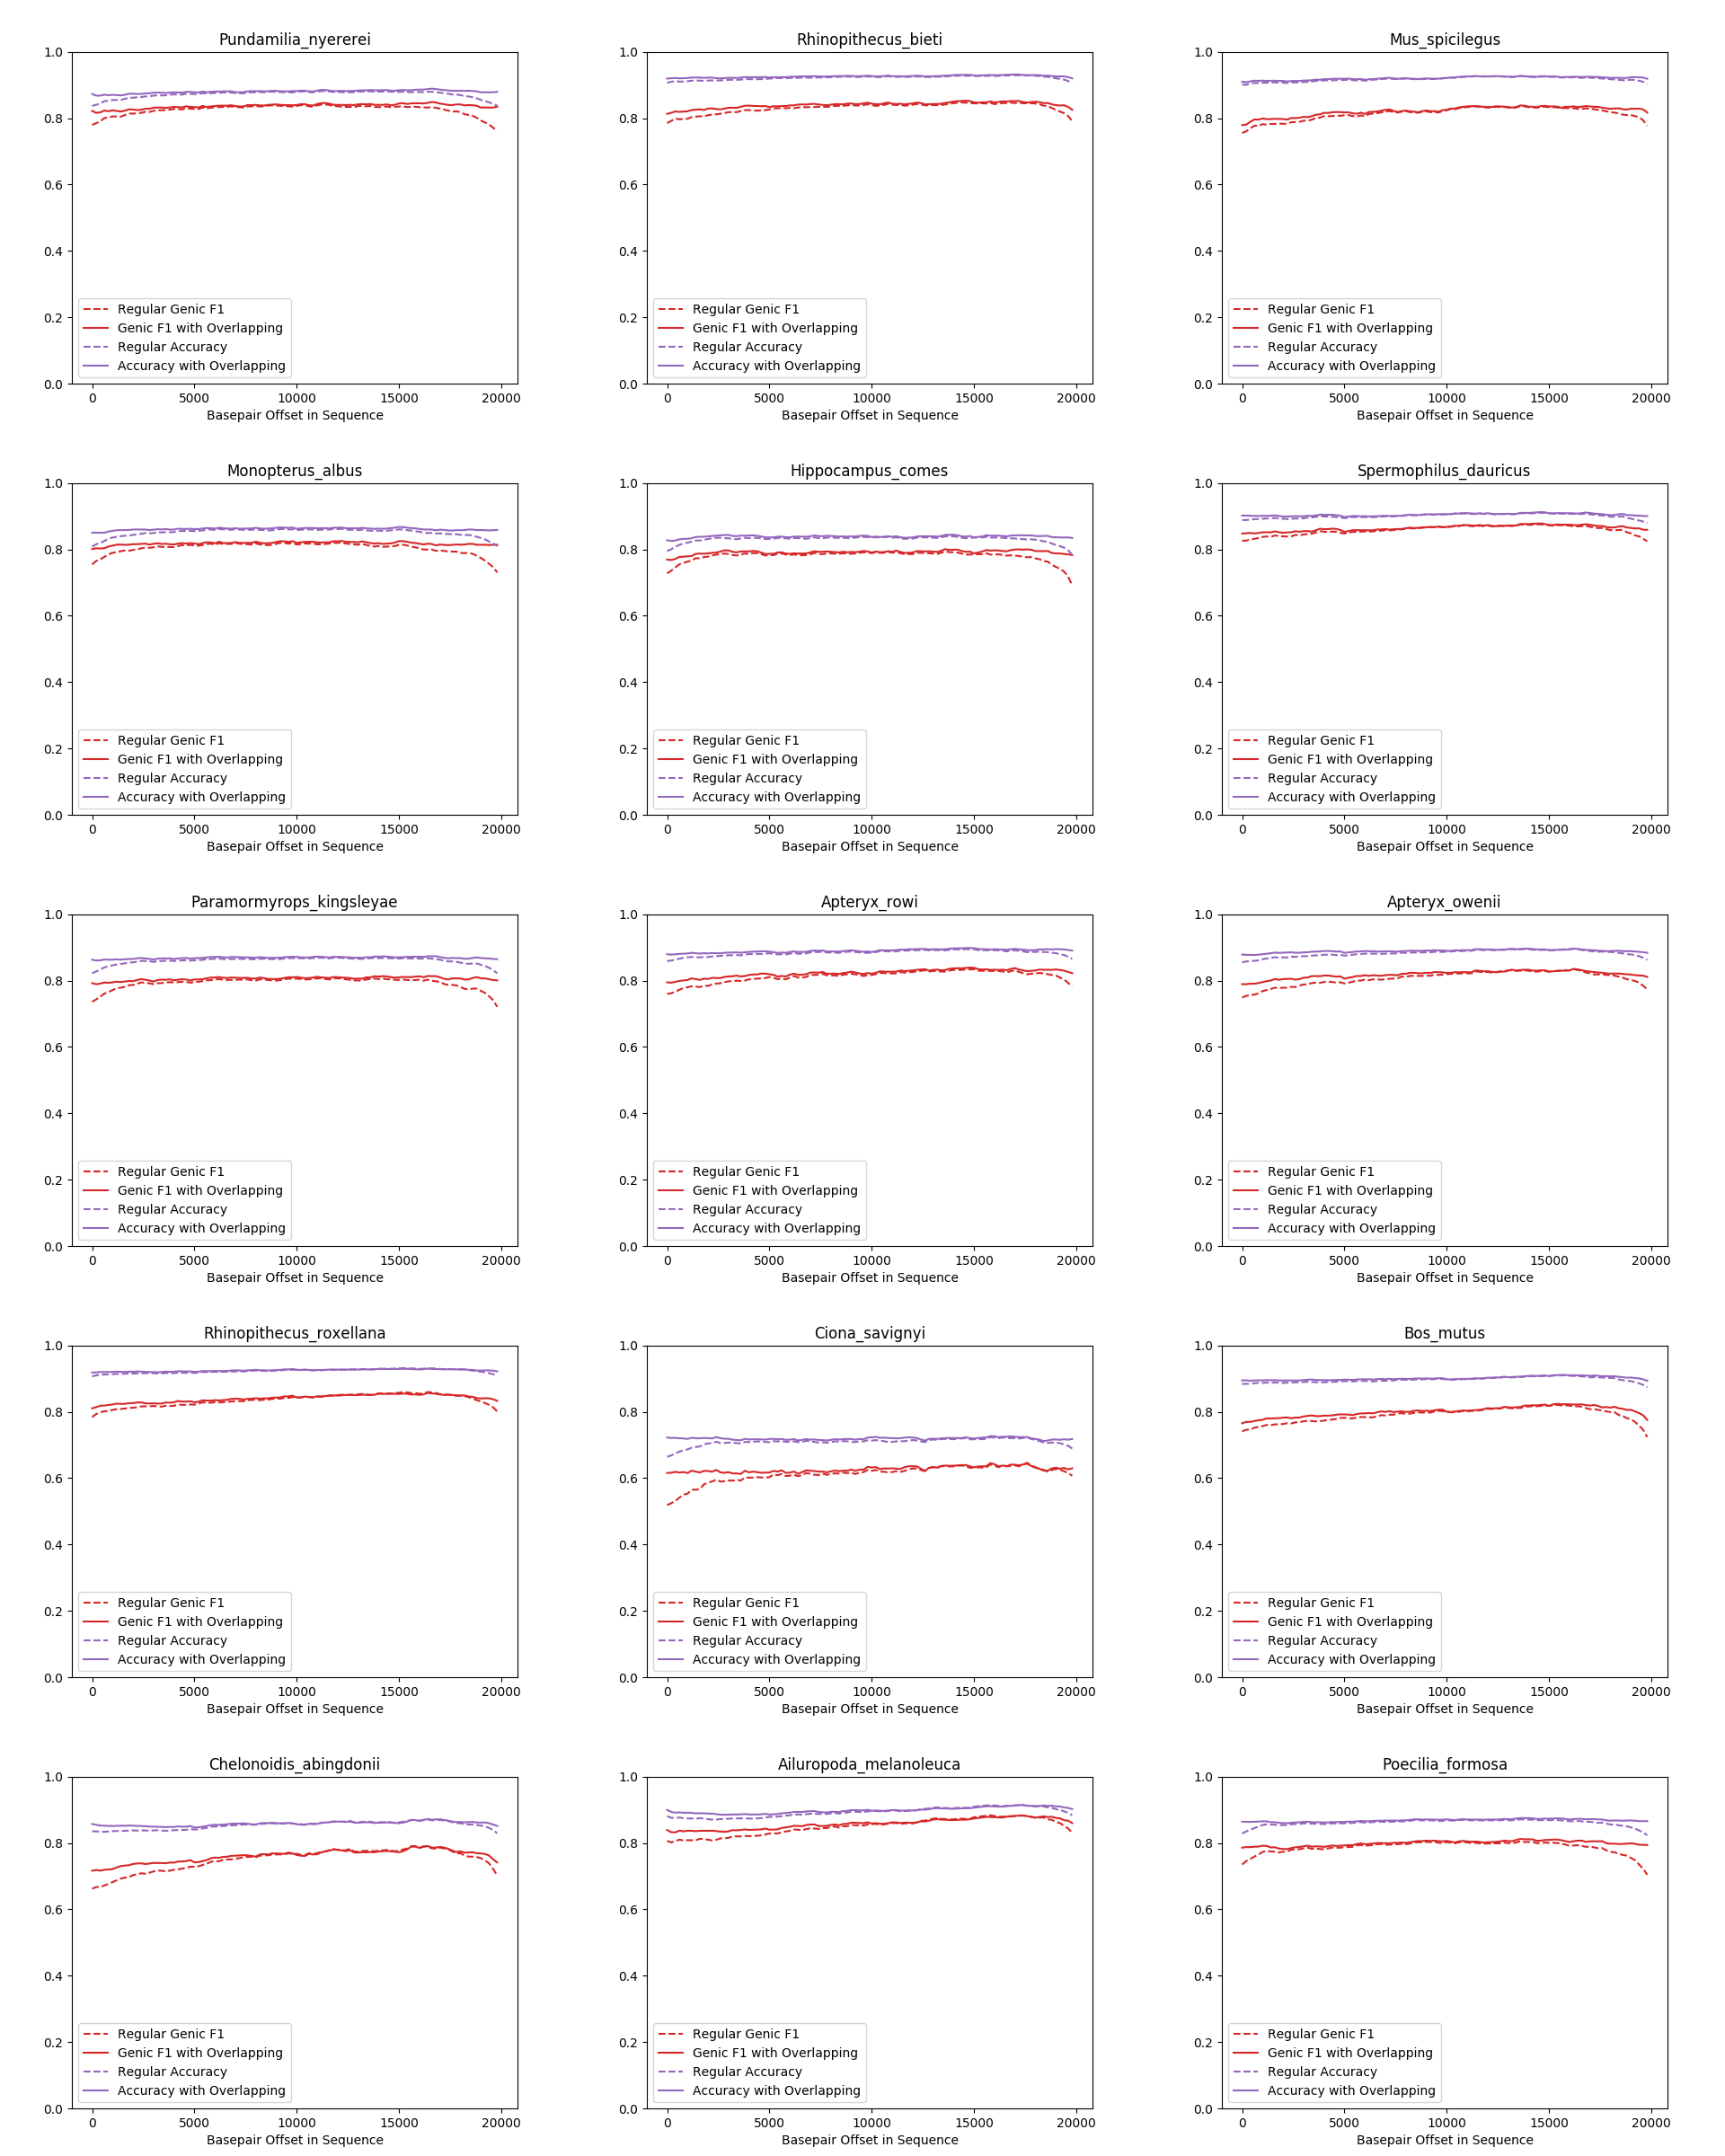
\includegraphics[width=1.2\textwidth]{images/overlapping/montage_animals10}}
\end{figure}
\begin{figure}[!h]
\centerline{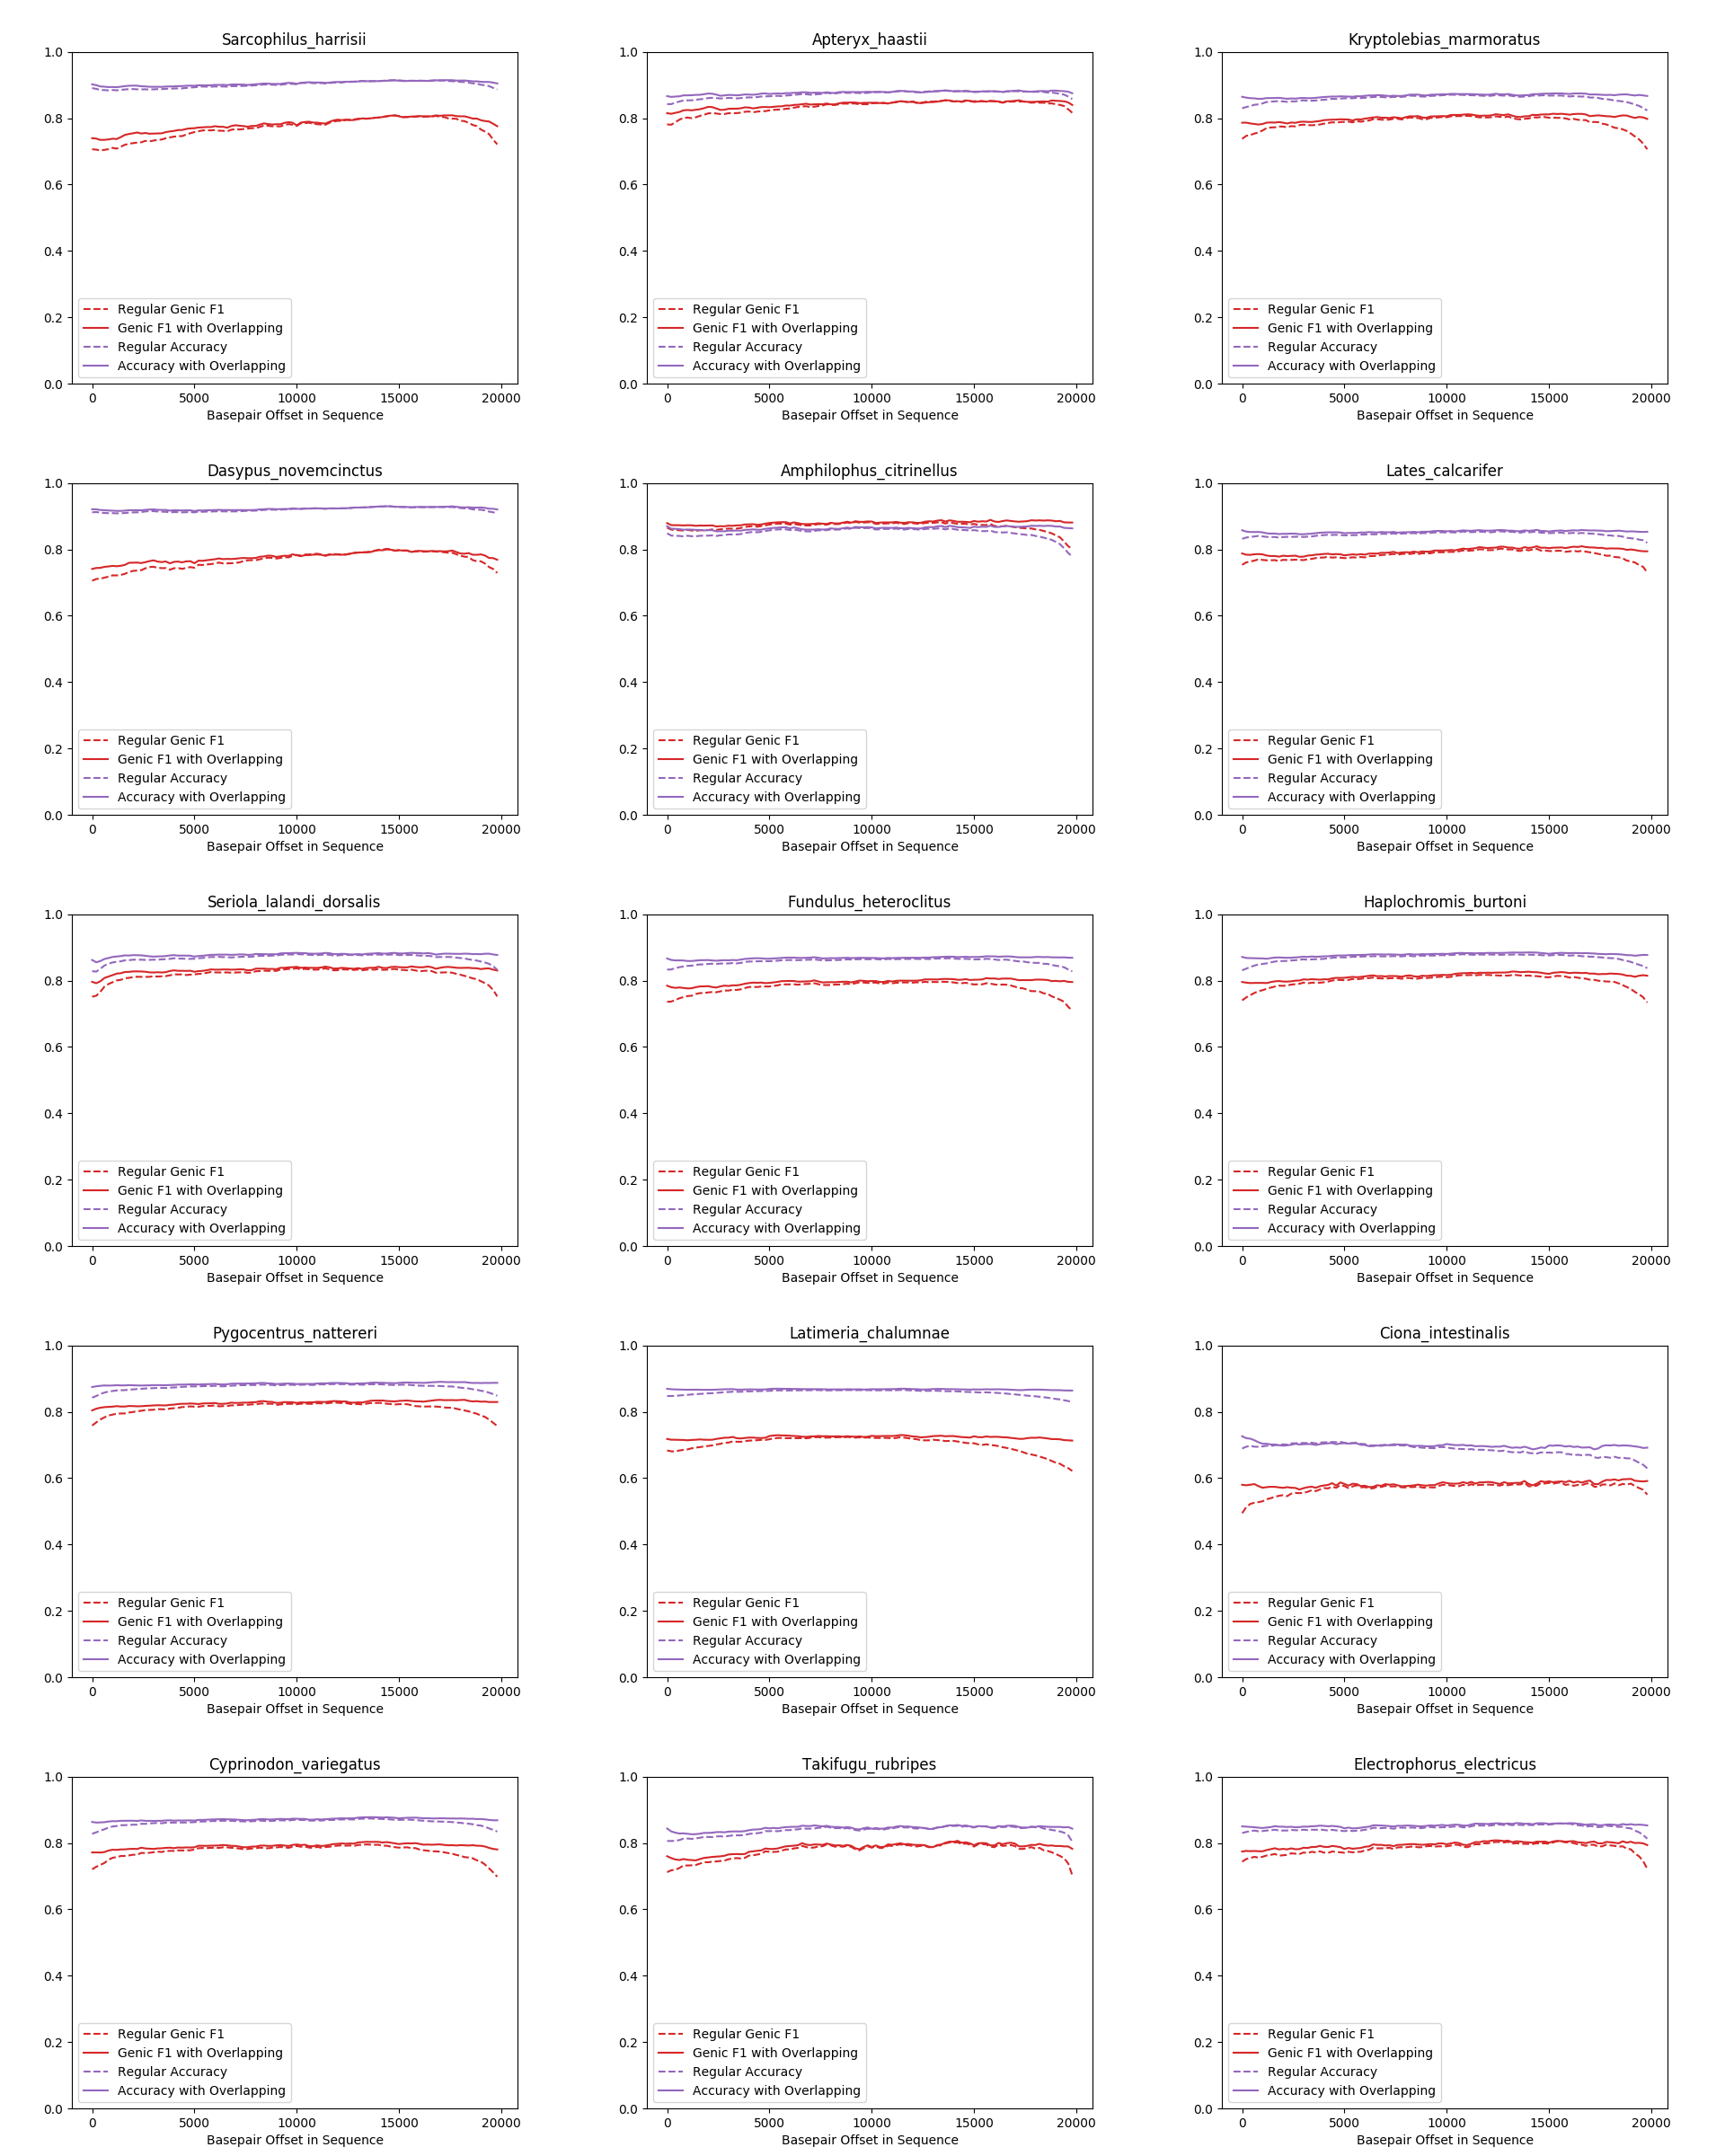
\includegraphics[width=1.2\textwidth]{images/overlapping/montage_animals11}}
\end{figure}
\begin{figure}[!h]
\centerline{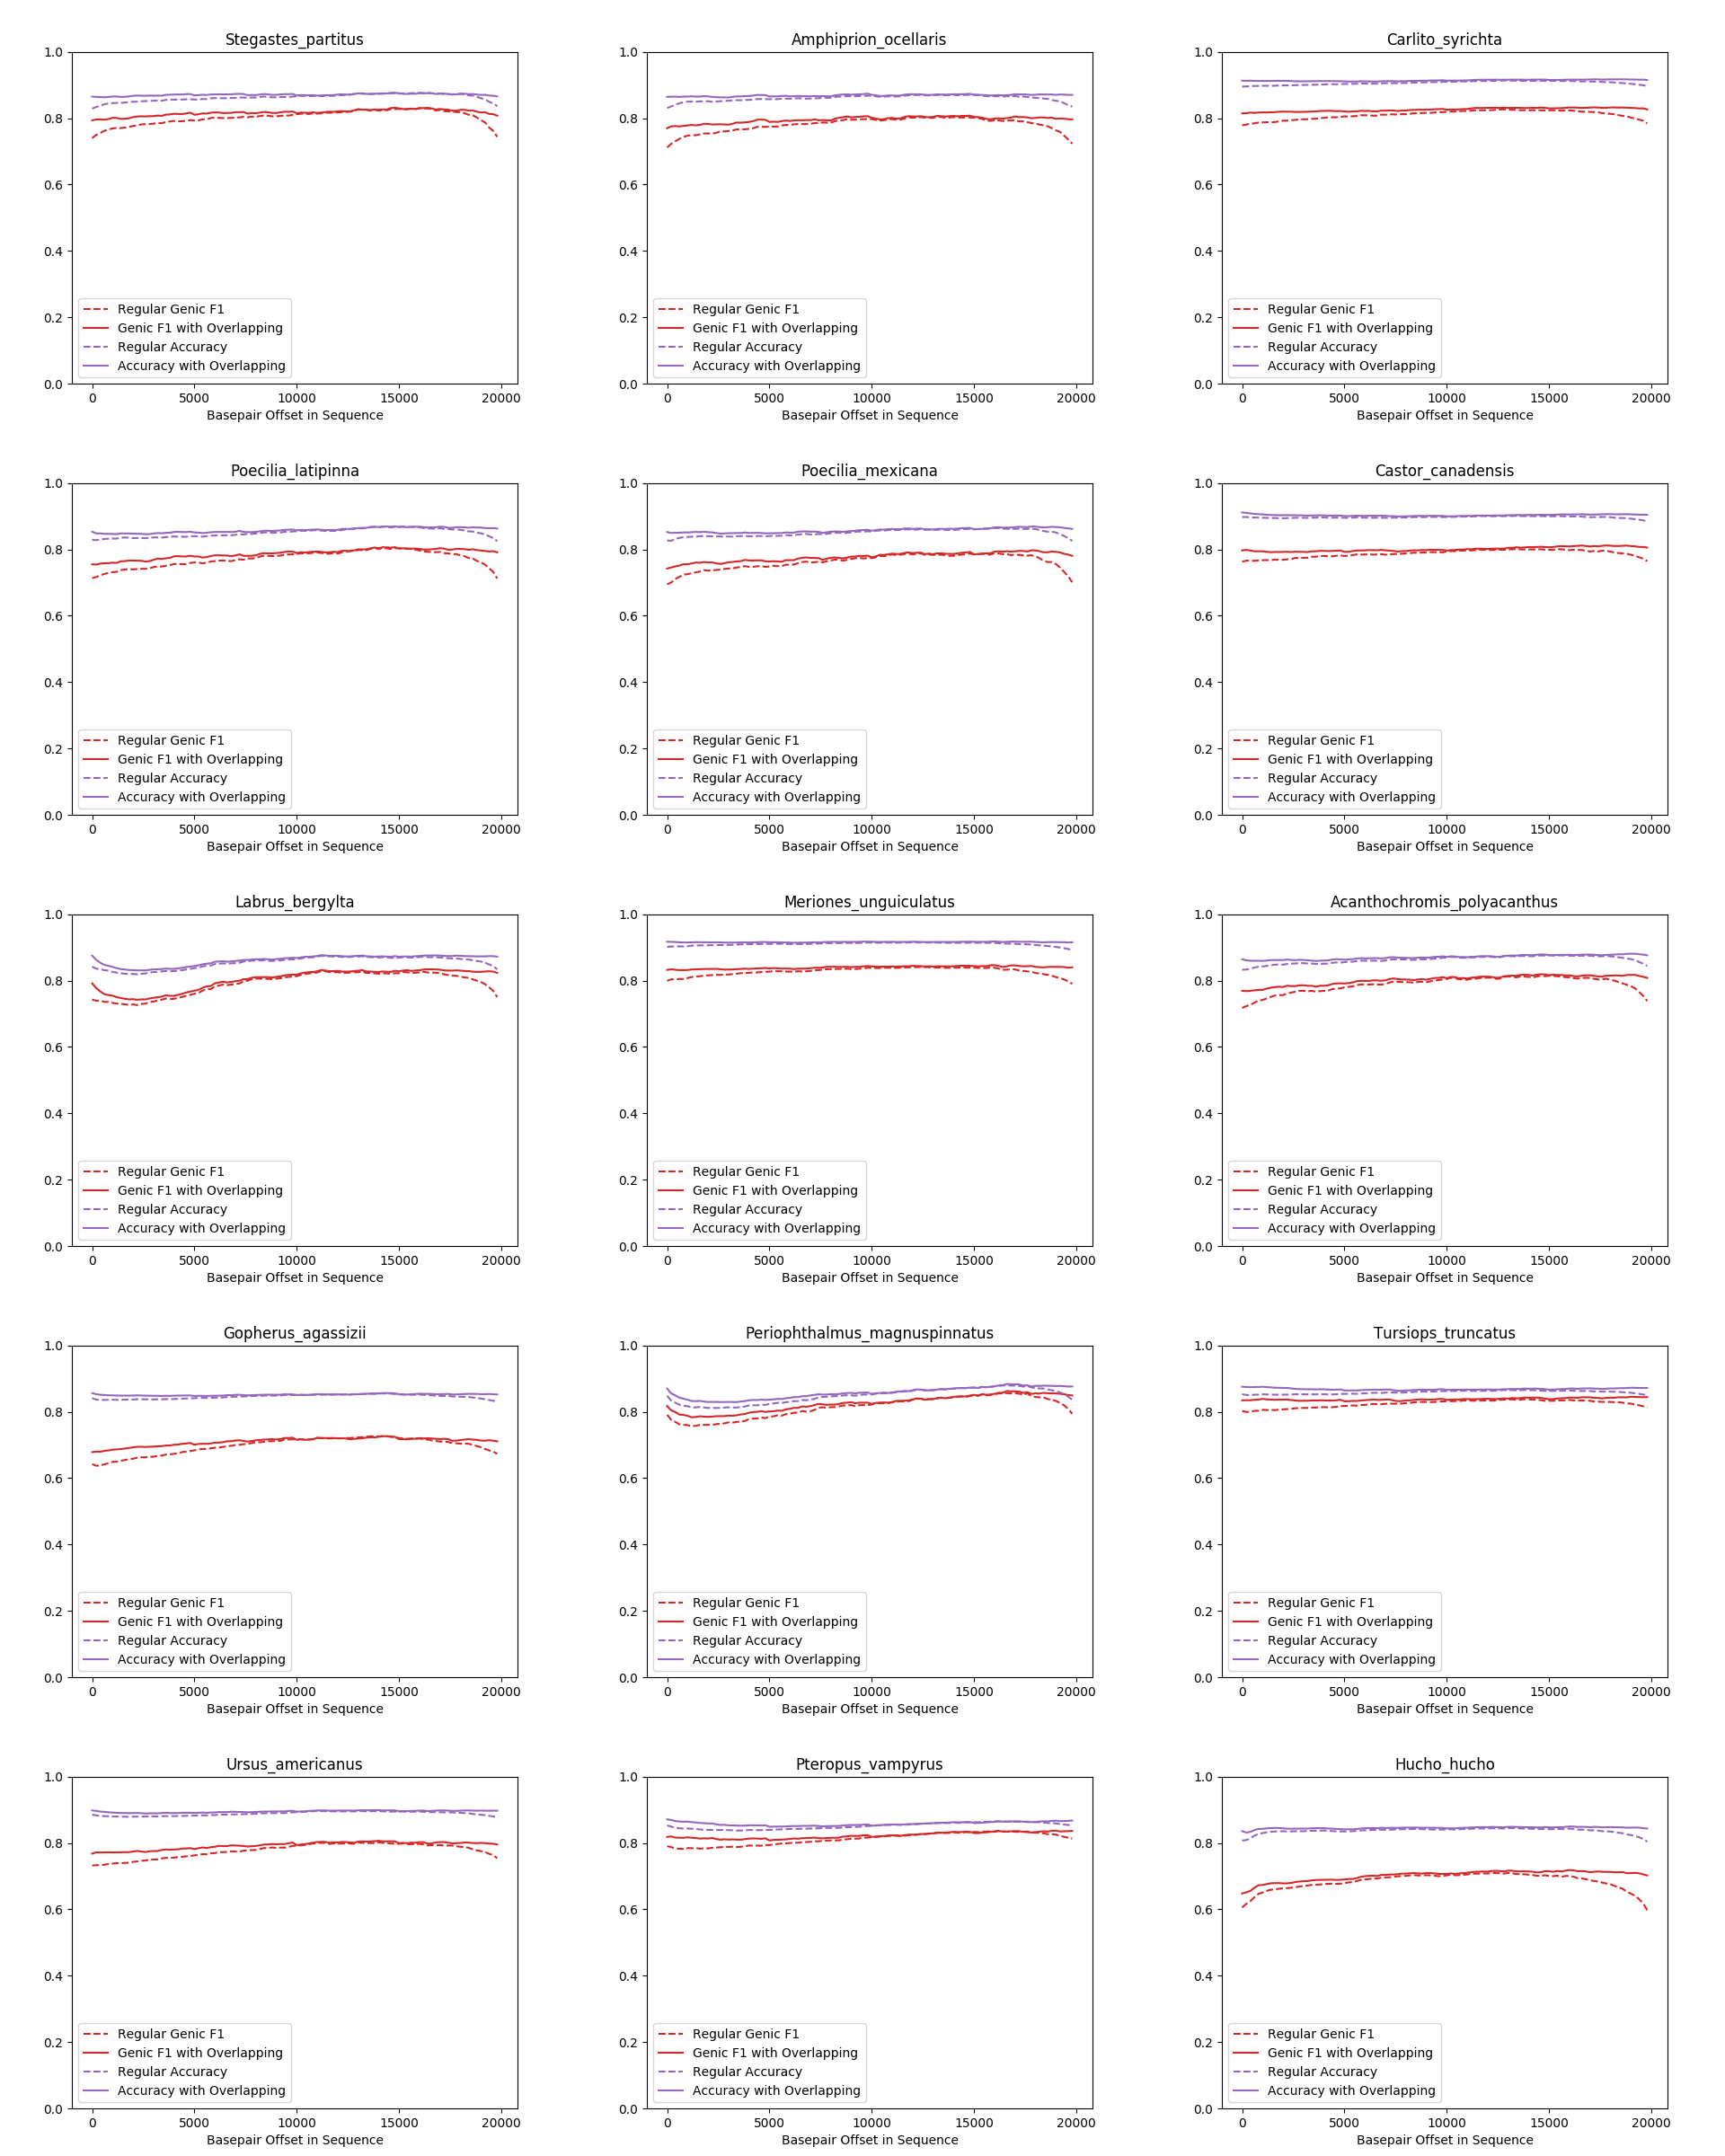
\includegraphics[width=1.2\textwidth]{images/overlapping/montage_animals12}}
\end{figure}
\begin{figure}[!h]
\centerline{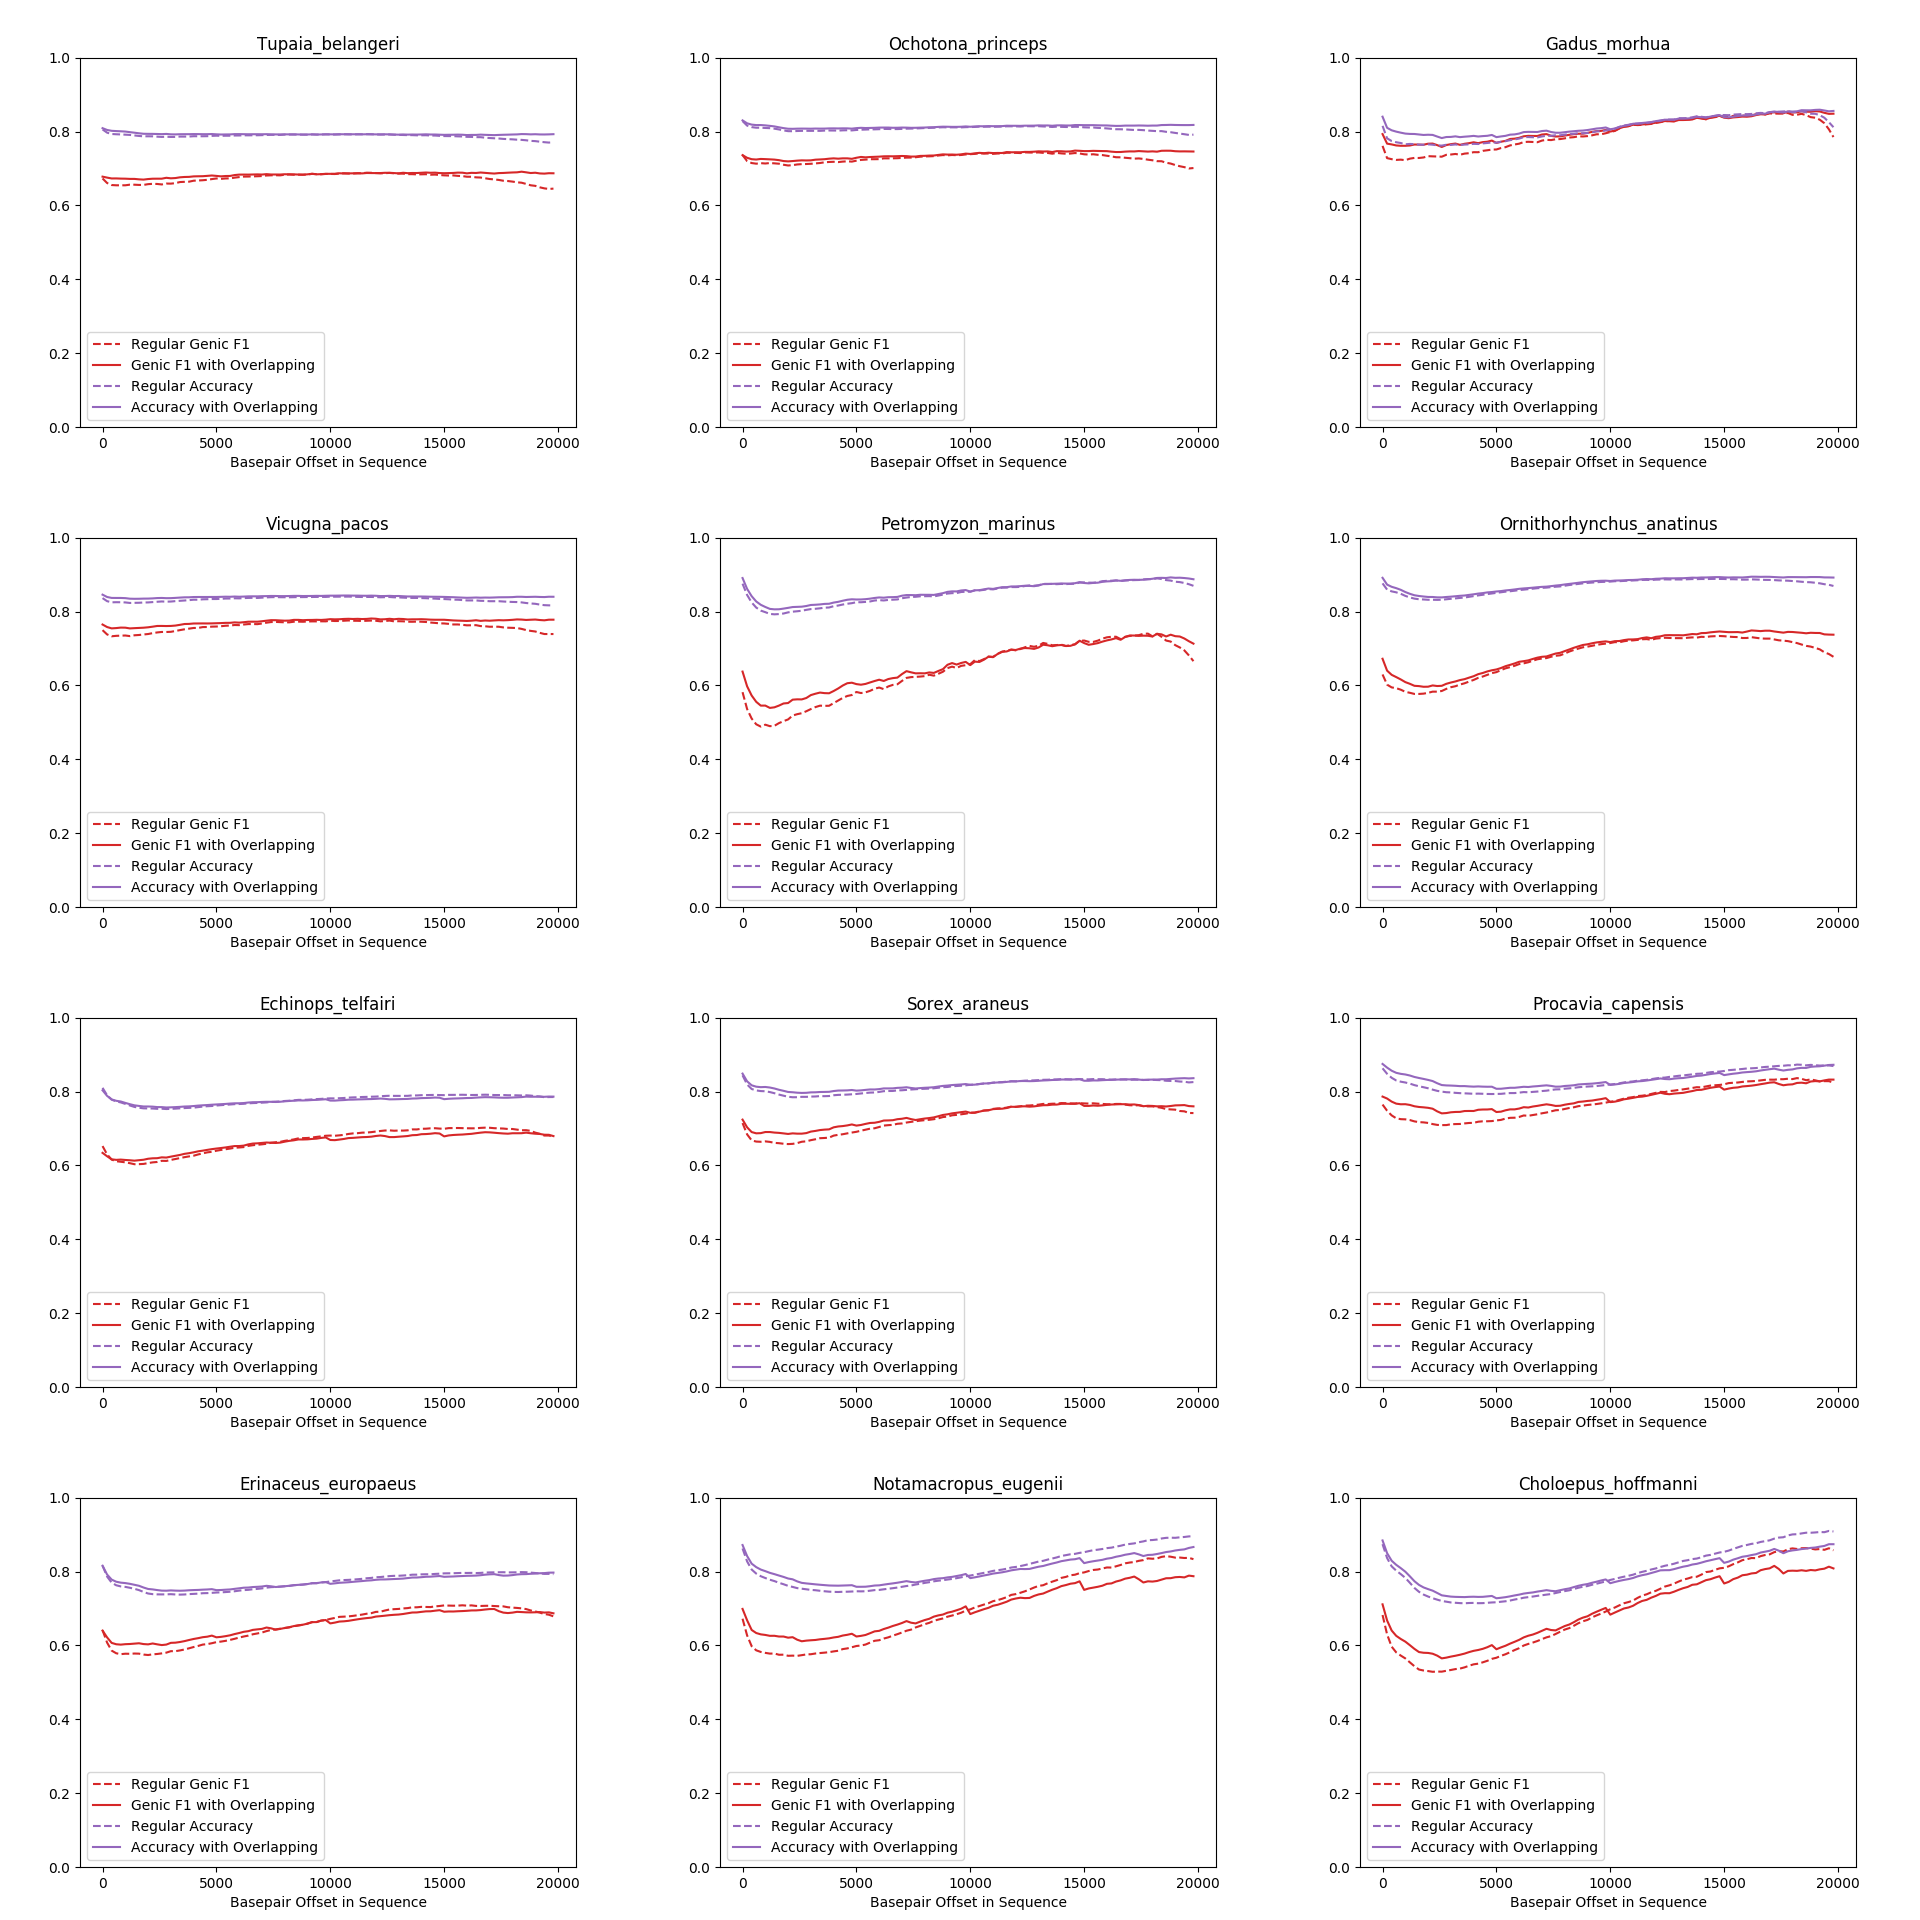
\includegraphics[width=1.2\textwidth]{images/overlapping/montage_animals13}}
\end{figure}

\clearpage
\subsection{Plants}

\begin{figure}[!h]
\centerline{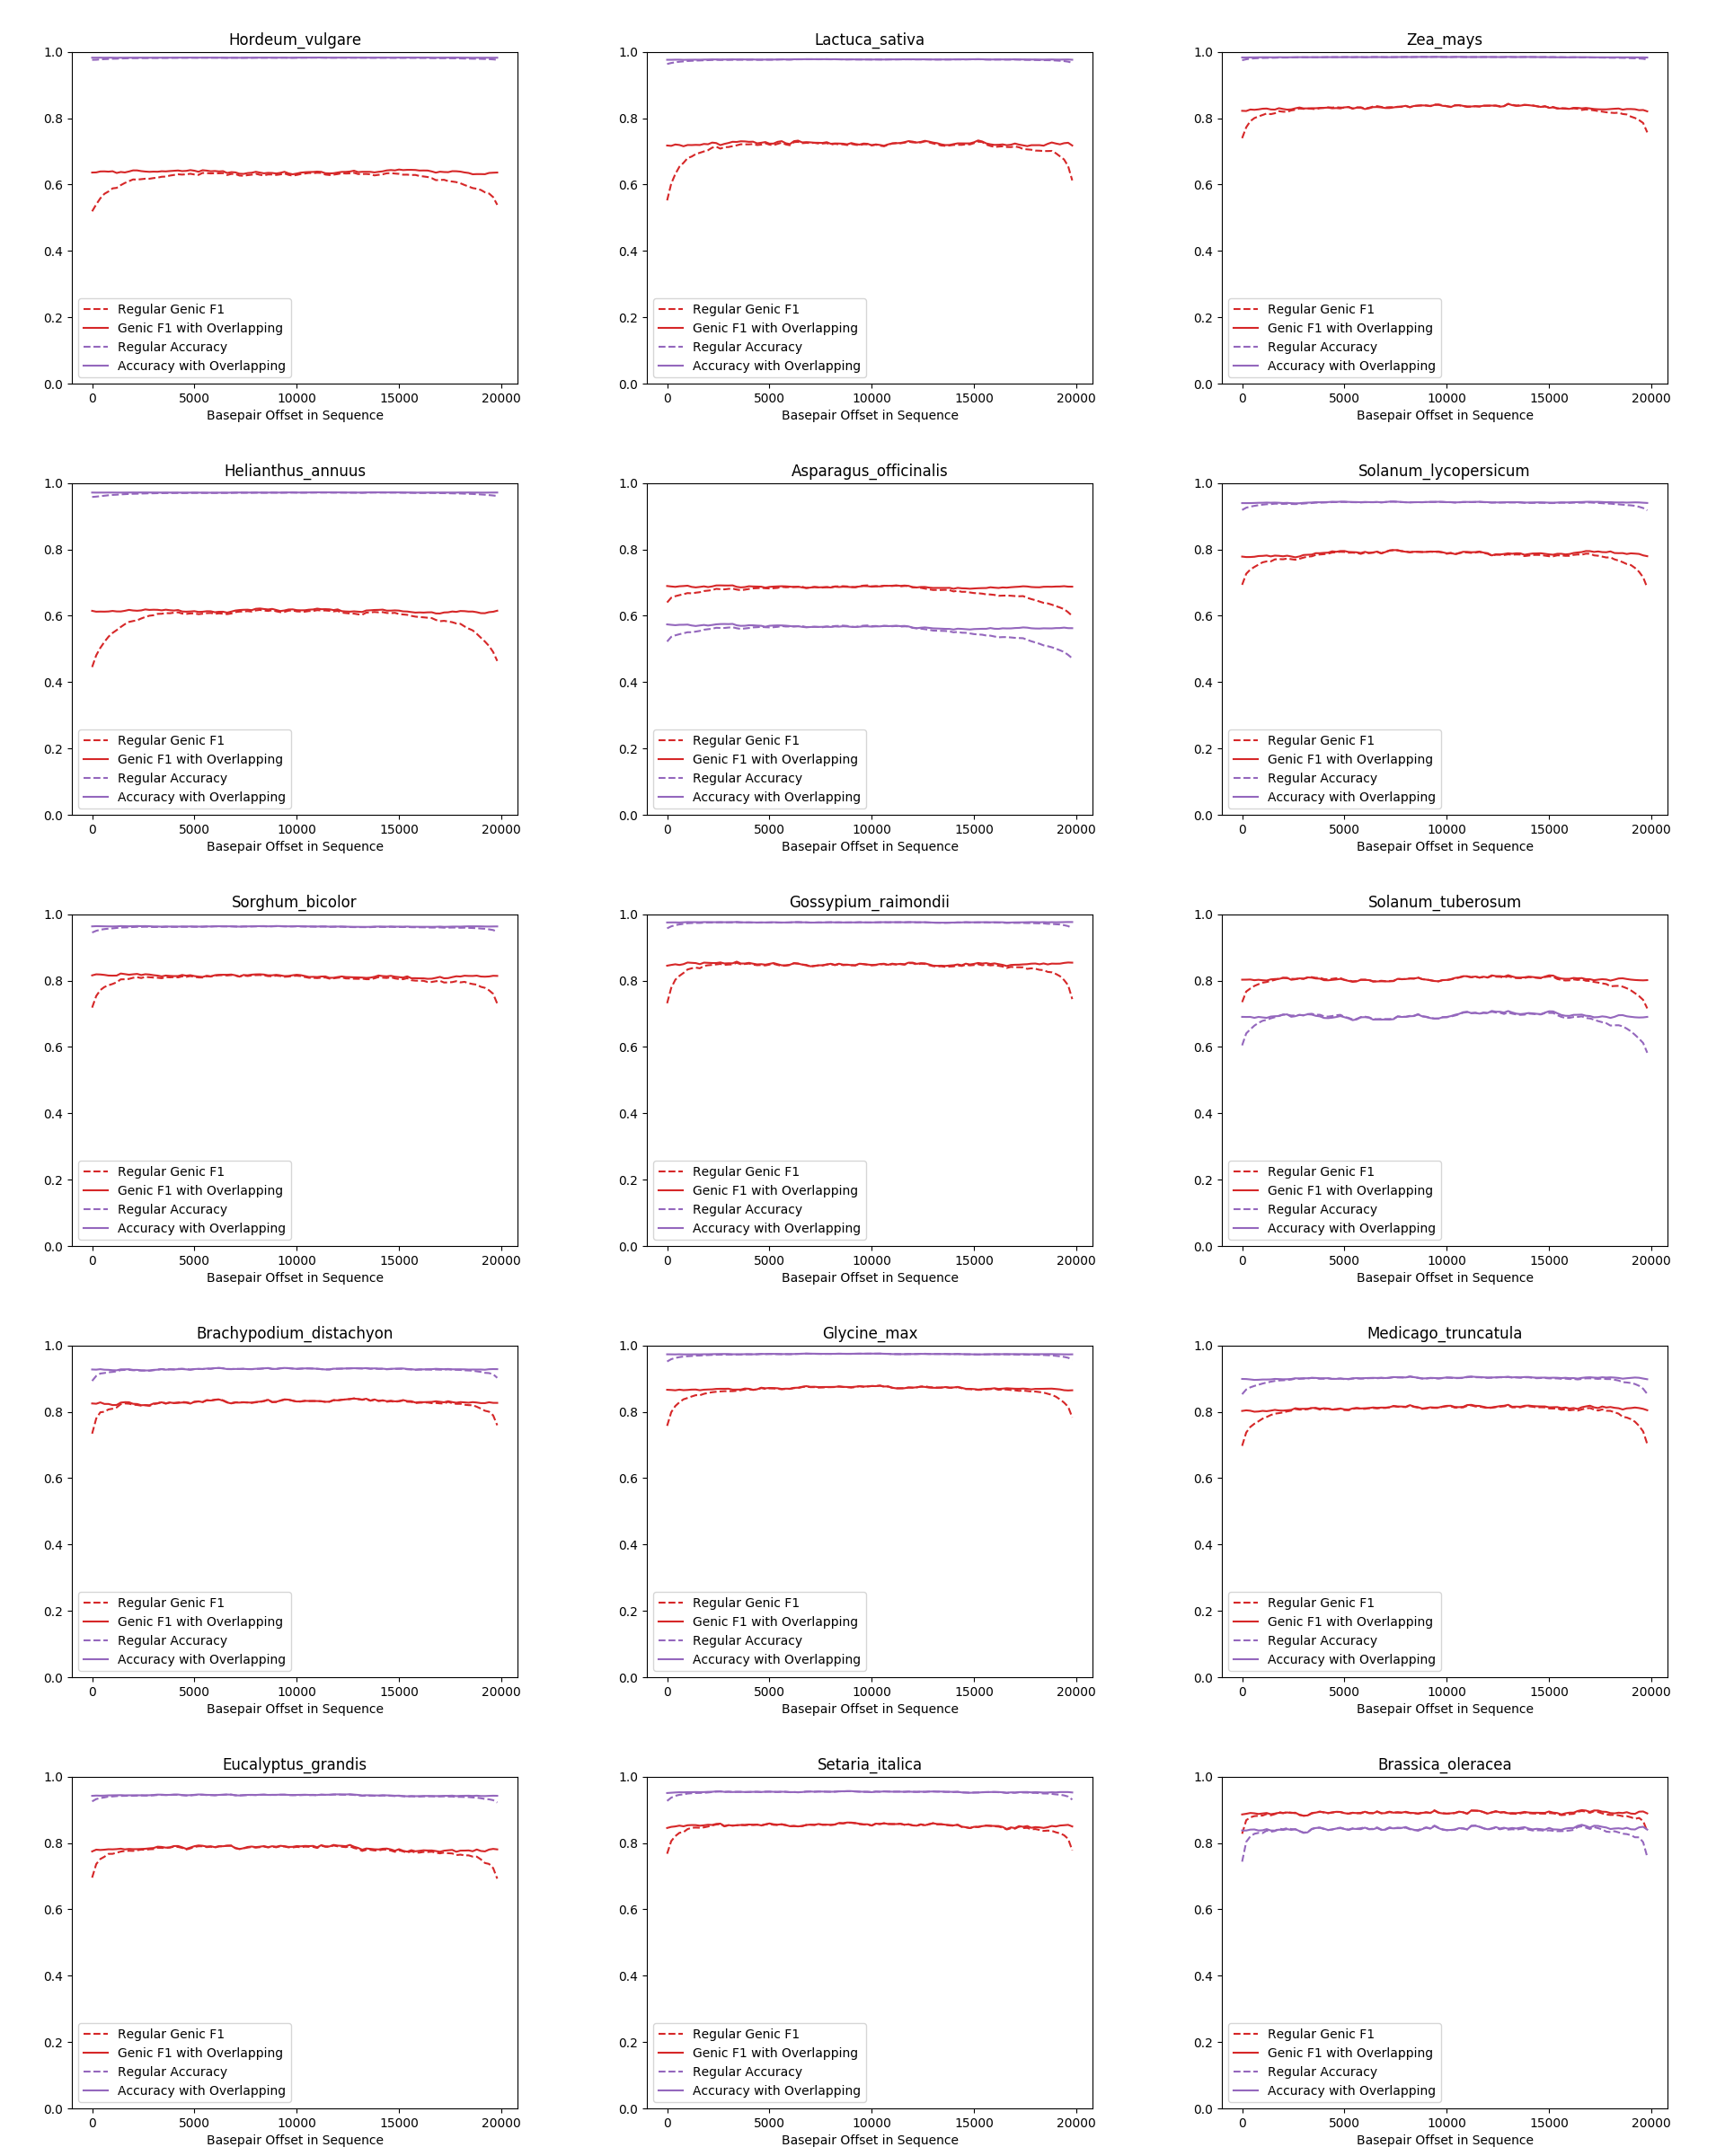
\includegraphics[width=1.2\textwidth]{images/overlapping/montage_plants1}}
\end{figure}
\begin{figure}[!h]
\centerline{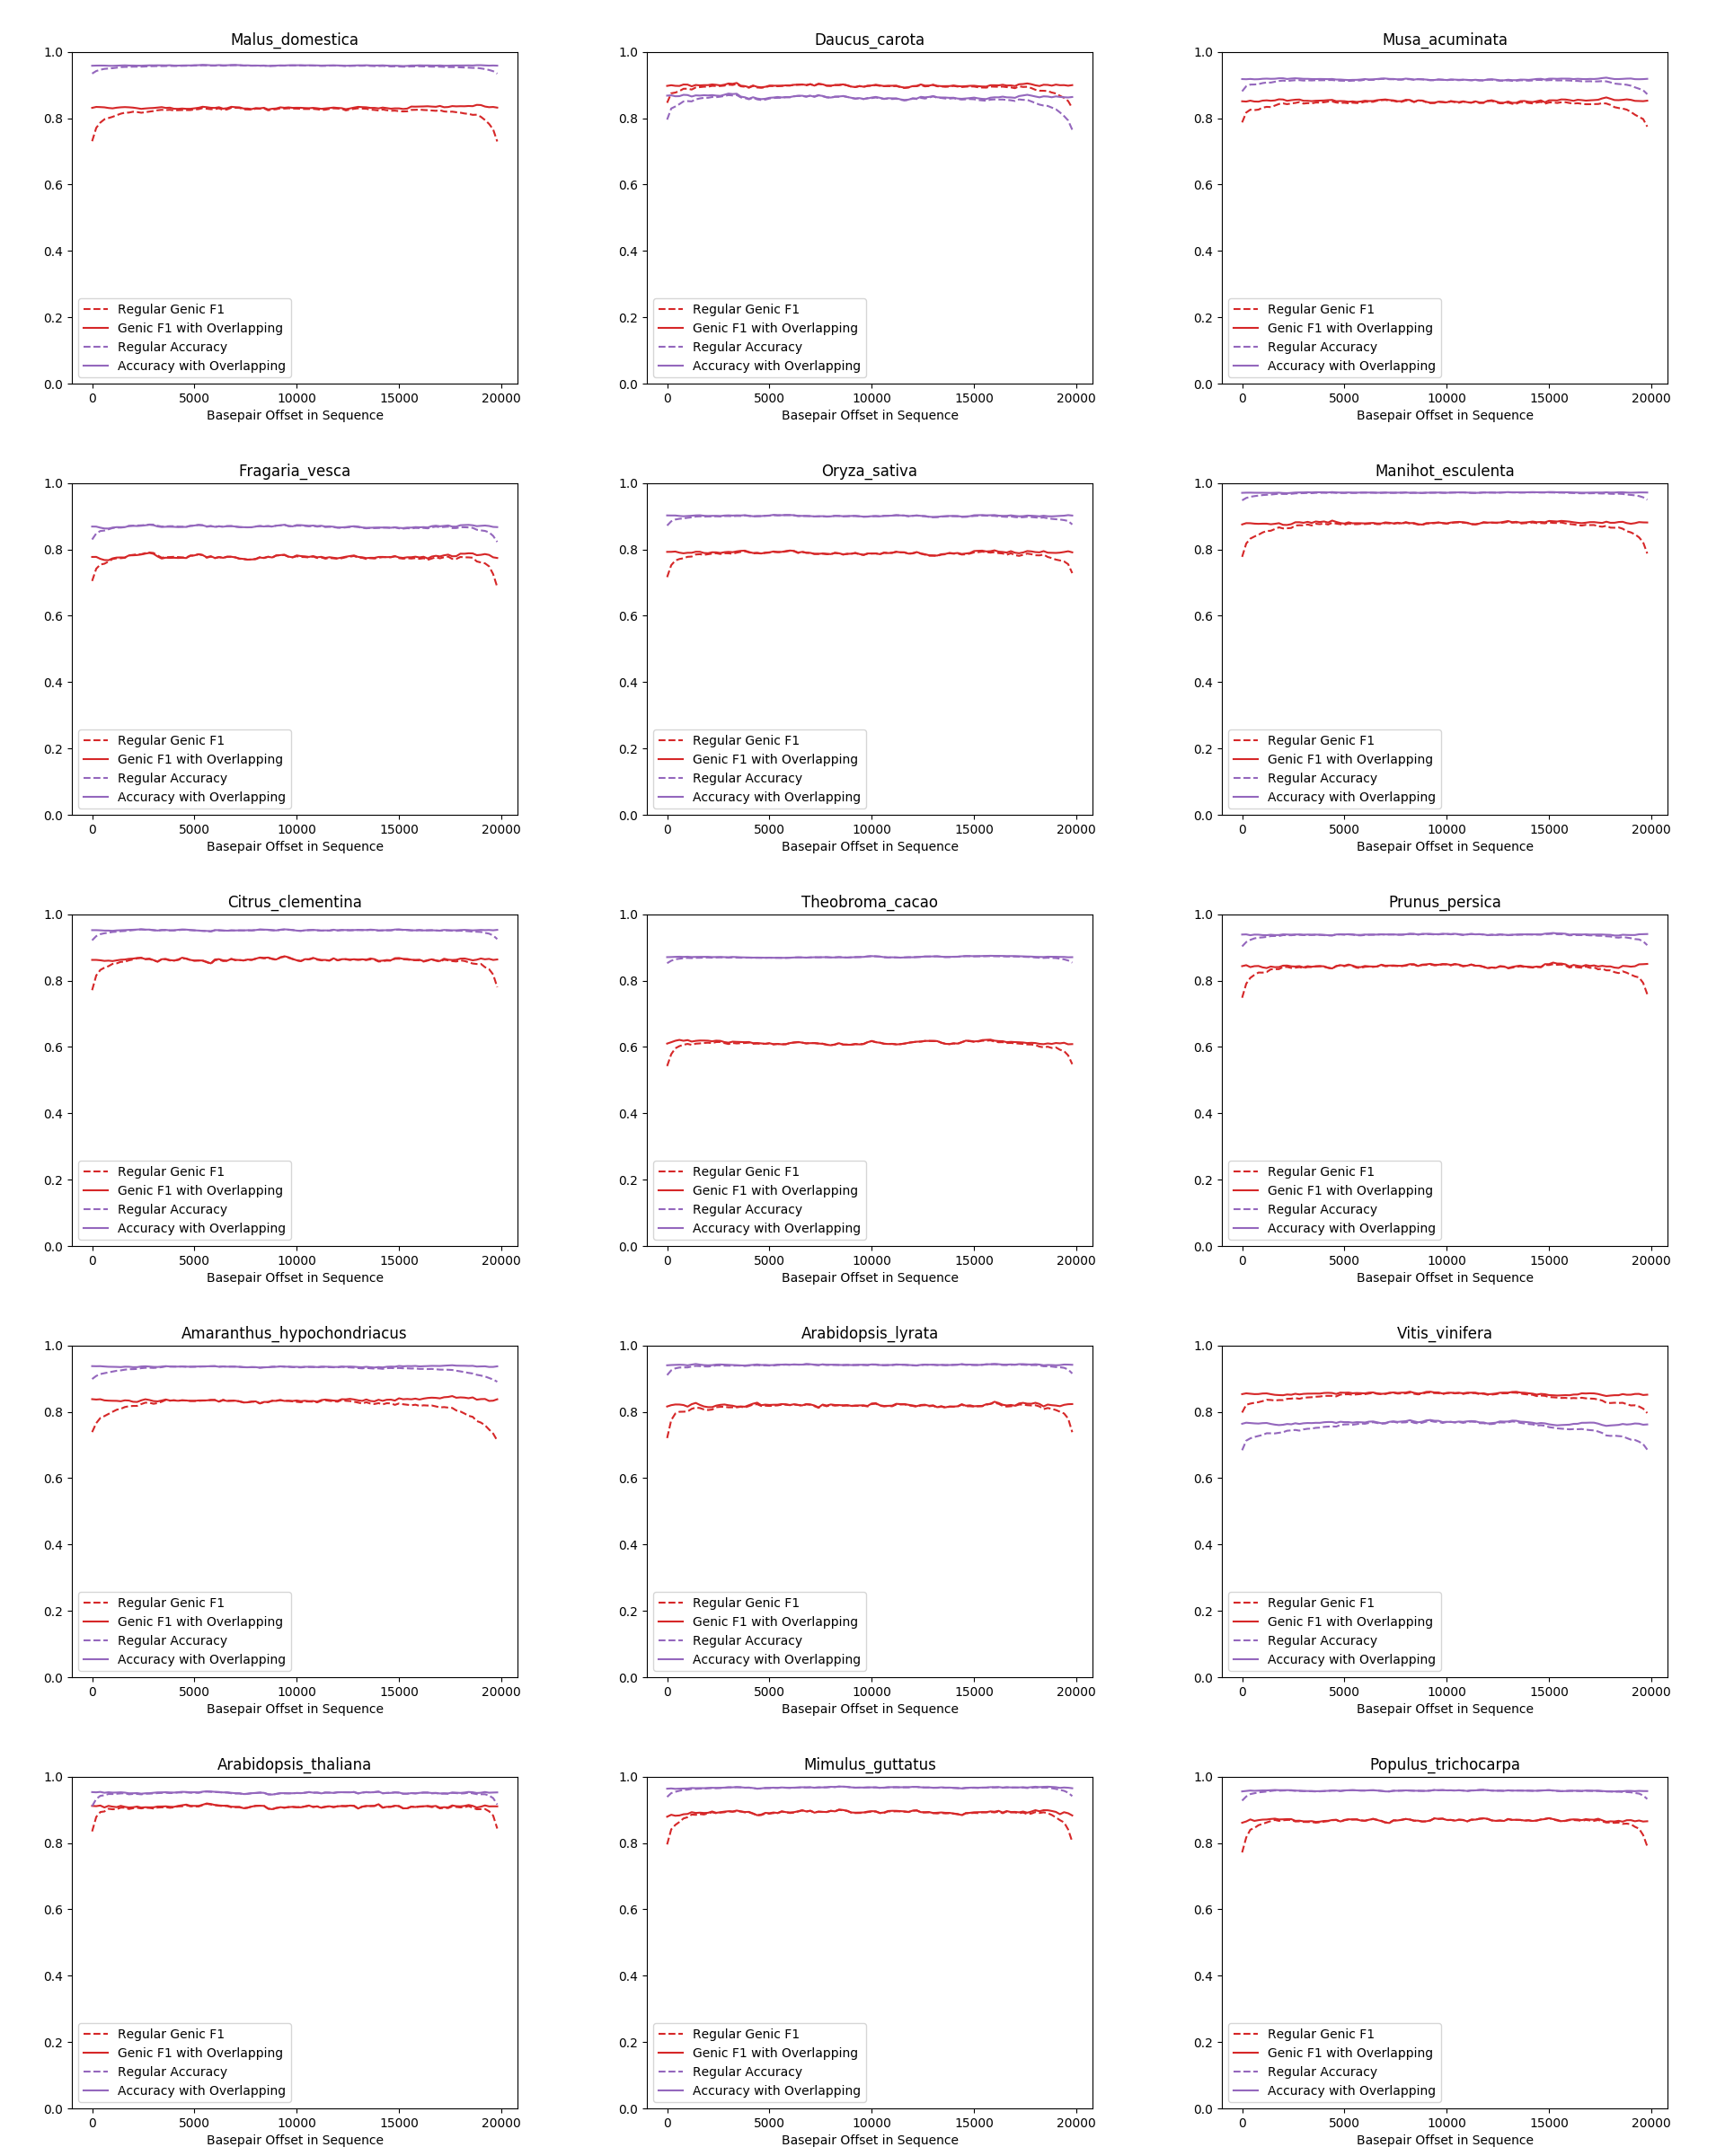
\includegraphics[width=1.2\textwidth]{images/overlapping/montage_plants2}}
\end{figure}
\begin{figure}[!h]
\centerline{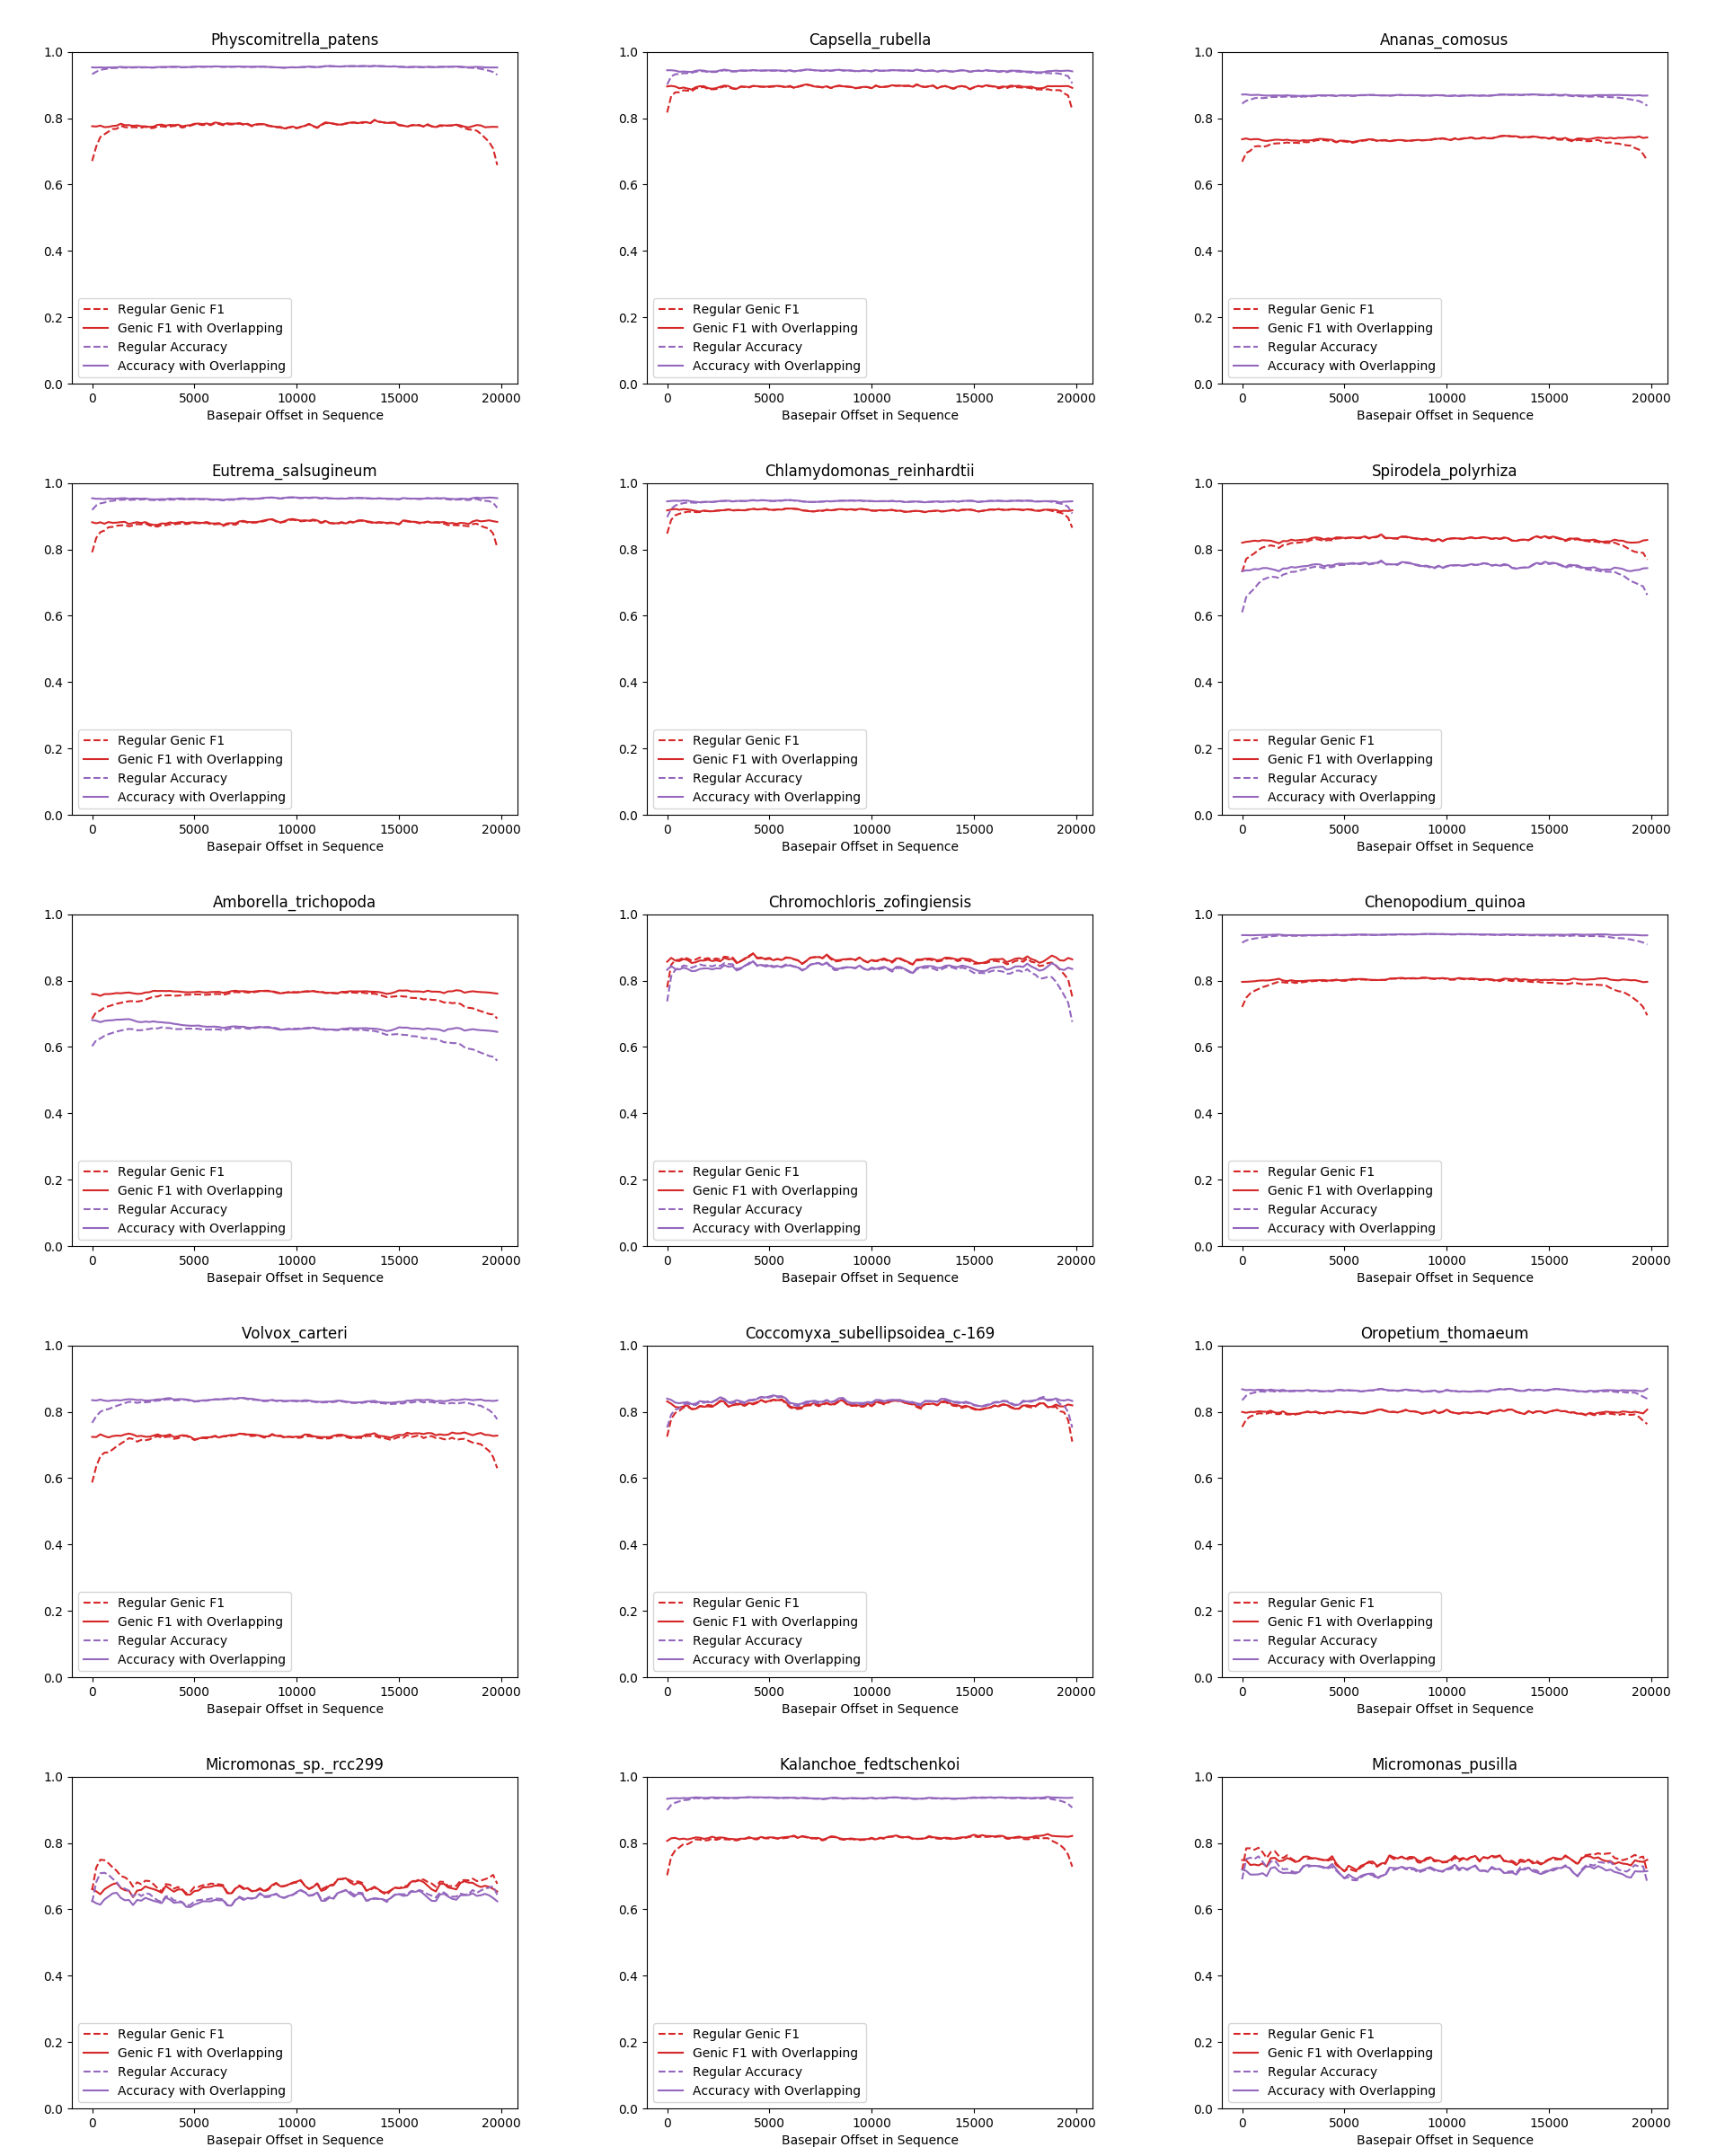
\includegraphics[width=1.2\textwidth]{images/overlapping/montage_plants3}}
\end{figure}
\begin{figure}[!h]
\centerline{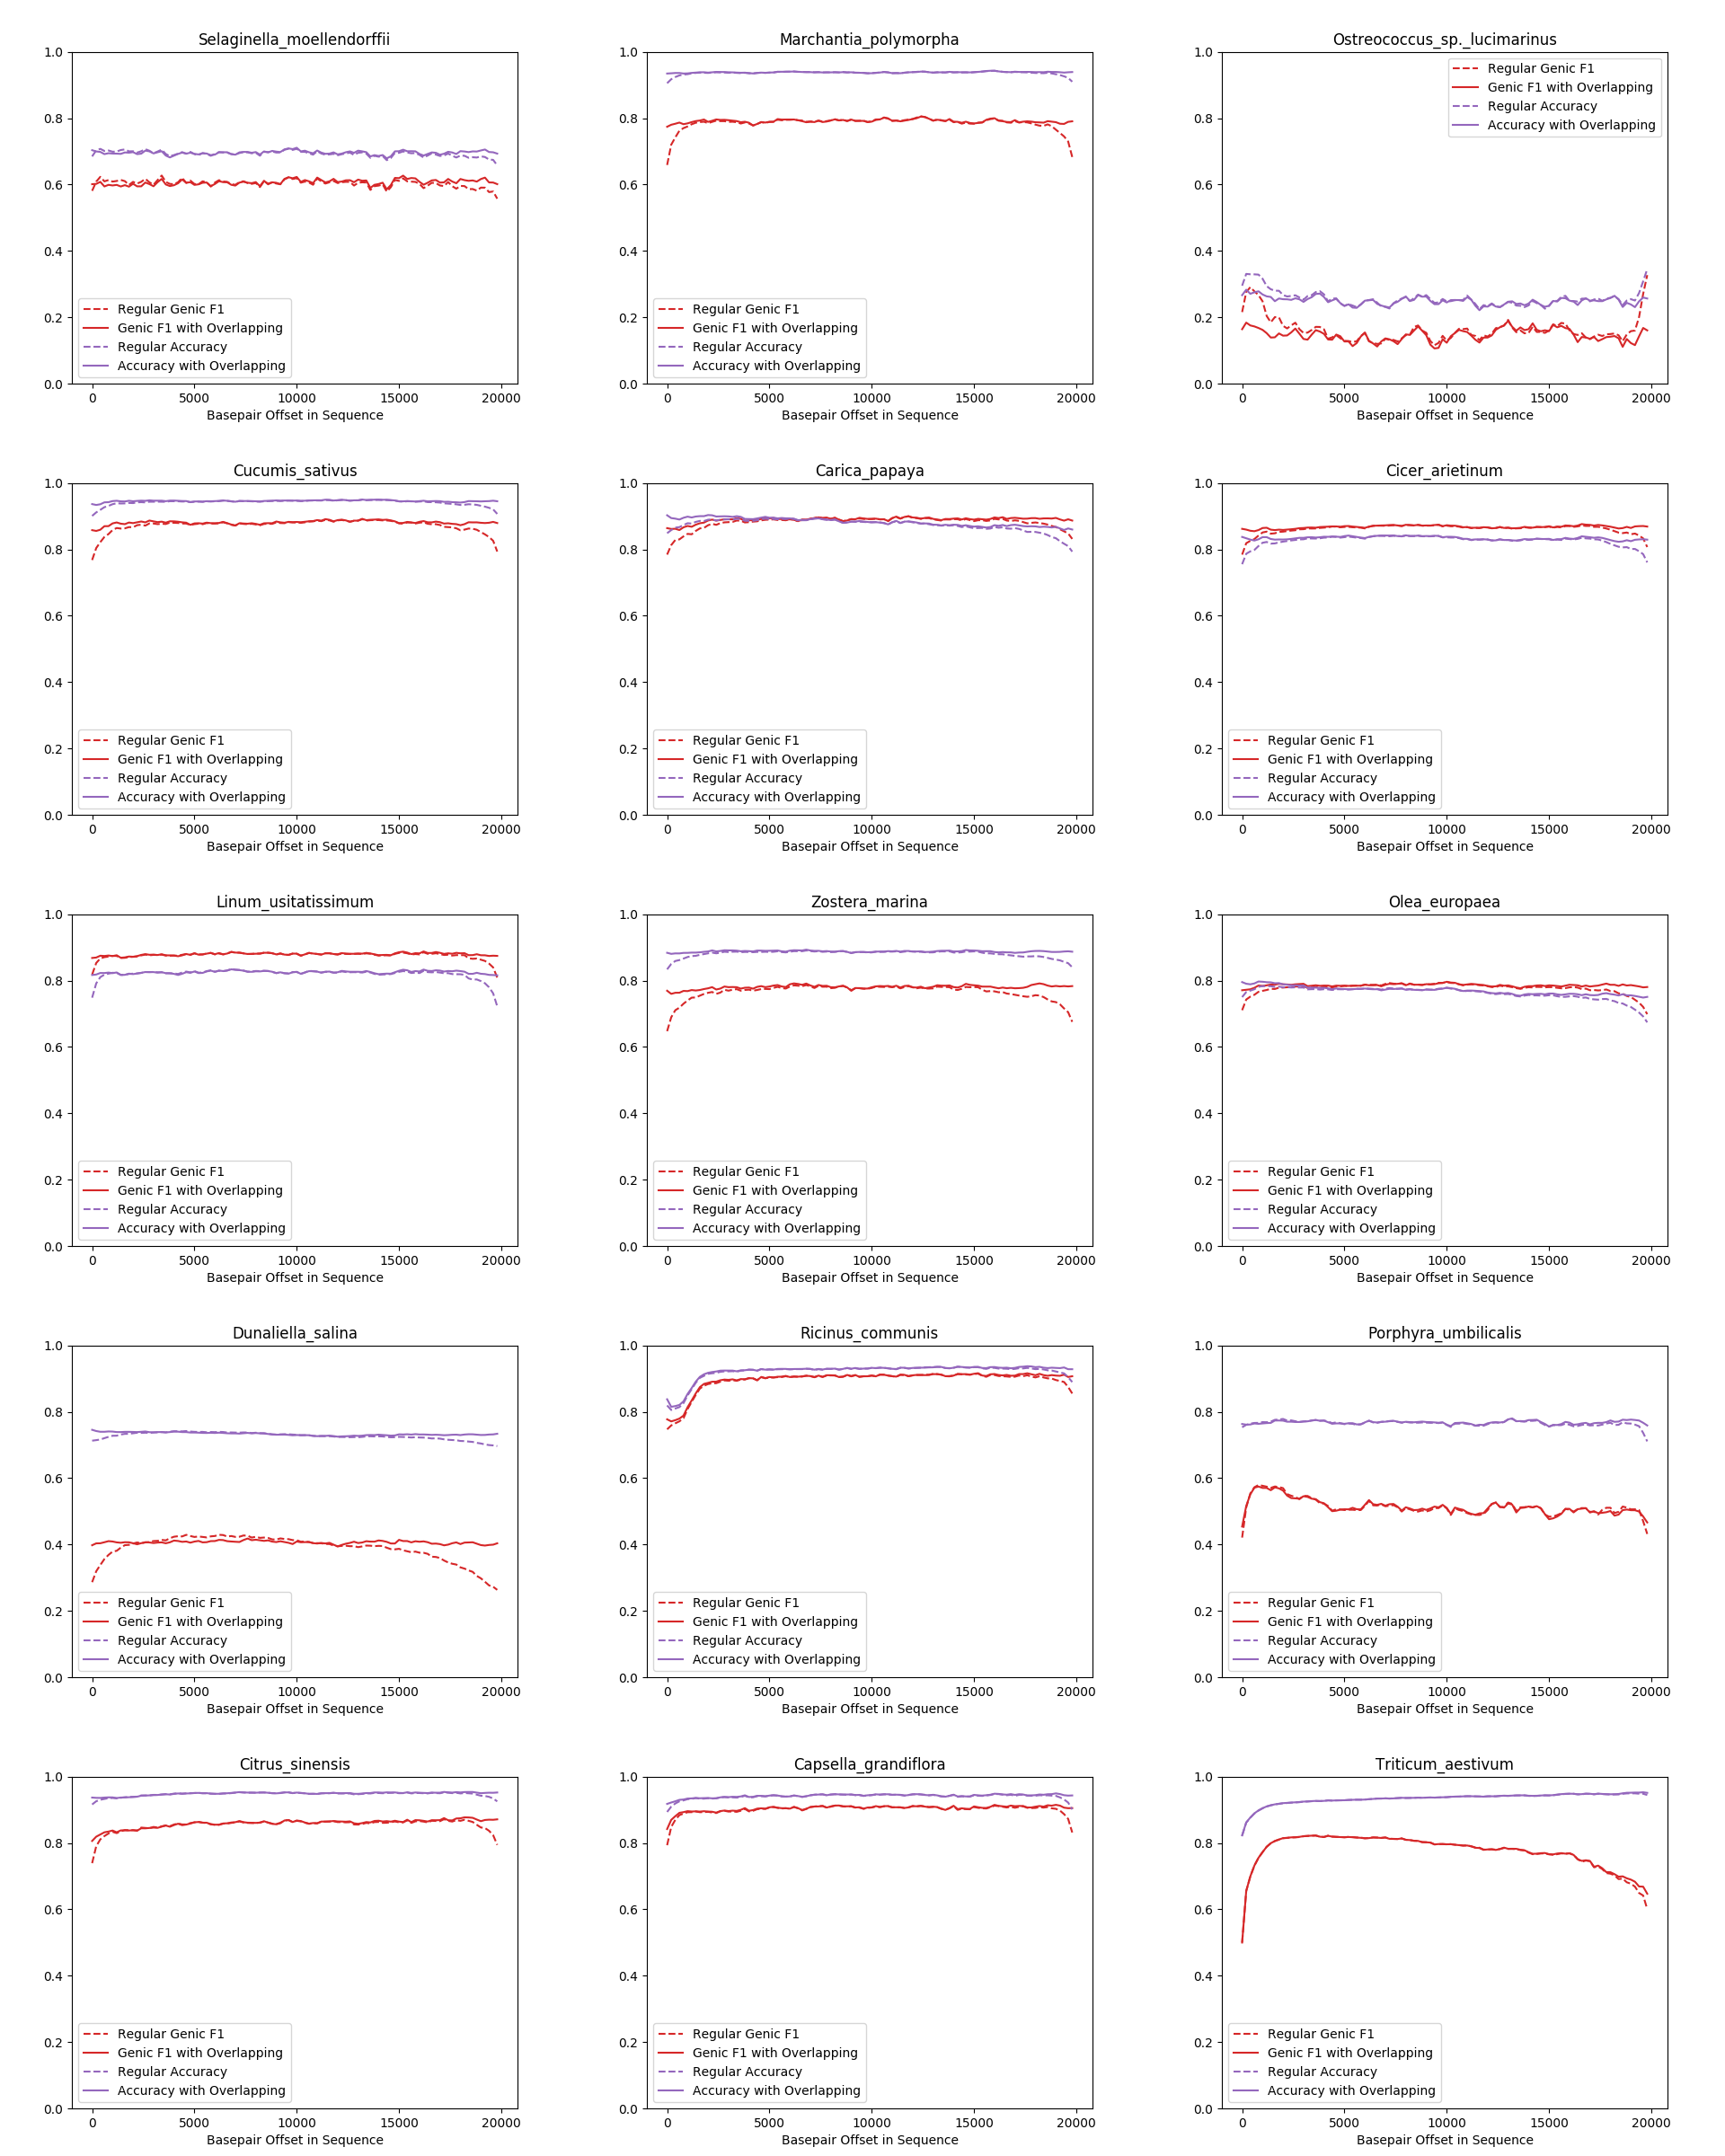
\includegraphics[width=1.2\textwidth]{images/overlapping/montage_plants4}}
\end{figure}

\clearpage
\section{Training Data statistics}
\label{sec:training_data}
\begin{table}[!h]
\renewcommand\thetable{S1}
\centering
\begin{tabular}{@{}lll@{}}
\hline
& Animals & Plants\\ [0.5ex]
\hline
Average genome size in Gbp& 2.489 (+- 2.073) & 0.914 (+- 0.934) \\
Average gene length & 25,672 (+- 16,605) & 3,509 (+- 906)\\
Geenuff error rate & 0.253 (+- 0.138) & 0.134 (+- 0.072) \\
Fraction of class Intergenic & 0.752 (+- 0.05) & 0.808 (+- 0.106) \\
Fraction of class UTR & 0.013 (+- 0.011) & 0.033 (+- 0.023) \\
Fraction of class CDS & 0.028 (+- 0.028) & 0.077 (+- 0.052) \\
Fraction of class Intron  & 0.207 (+- 0.023) & 0.083 (+- 0.037) \\
\hline
\end{tabular}
\caption{The description of Table [?] applies here as well.}
\end{table}


\newpage
\section{Dilated CNN Baseline Network Search}
\begin{table}[!h]
\renewcommand\thetable{S1}
\centering
\begin{tabular}{@{}ll@{}}
\hline
Parameter & Search Space\\ [0.5ex]
\hline
Kernel Size & \{4, 8, 12, 16\}\\
Initial Filter Depth & \{32, 64, 96, 128\}\\
Number of Layers Before Doubling Filter Count & \{1, 2\}\\
Dilation Multiplier & \{2, 3\}\\
Number of Convolutional Layers & \{2, 3, 4, 5, 6, 7, 8\}\\
Number of Hidden Fully Connected (FC) Layers & \{0, 1, 2\}\\	
Dropout Used on FC and Final Conv Layer Output & \{0.0, 0.01, 0.1, 0.2, 0.3\}\\
Learning Rate & \{1e-3, 1e-4\}\\
\hline
\end{tabular}
\caption{Above are all parameters used during neural architecture search for the dilated CNN baseline. The same overall space was used for plant and animal data. We did, however, run multiple distinct searches that sometimes only operated over a subset of the given parameters. This was done as those seemed to be the most promising. We for example restricted the search space of the number of LSTM layers to the highest 3 values in later runs. Decisions were guided by the Genic F1 on the validation set of exactly the same data we trained our final LSTM models with. Runs with a Genic F1 below 0.5 after 10 epochs were stopped and the overall maximum epoch was 15. The performances seemed to be leveling off well before that. The batch size used for almost all runs was 32, the dilation was capped to 81 and the size of each fully connected layer was fixed at 128. New parameters where chosen at random. The implementation and parameter space is very roughly based on \citep{gupta2017dilated} and can be found in the Helixer source code repository. In total, we trained 30 models for the animals and 48 with the plant data.}
\end{table}

\begin{table}[!h]
\renewcommand\thetable{S1}
\centering
\begin{tabular}{@{}lll@{}}
\hline
Parameter & Animals & Plants\\ [0.5ex]
\hline
Kernel Size & 16 & 16\\
Initial Filter Depth & 96 & 32\\
Number of Layers Before Doubling Filter Count & 2 & 2\\
Dilation Multiplier & 3 & 3\\
Number of Convolutional Layers & 6 & 8\\
Number of Hidden Fully Connected (FC) Layers & 2 & 0\\
Dropout Used on FC Output & 0.0 & 0.0\\
Learning Rate & 1e-4 & 1e-3\\
\hline
\end{tabular}
\caption{The parameters of the dilated CNN model that performed the best according to the Genic F1 of the validation data of the respective training genomes. The best animal model has circa 4.6 million parameters; the best plant model around 2.1 million.}
\end{table}



\renewcommand\refname{Supplemental Reference}
\bibliographystyle{natbib}
\bibliography{literature}

\end{document}
